\documentclass[a4paper,12pt]{extarticle}
\usepackage{geometry}
\usepackage[T2A,T1]{fontenc}
\usepackage[utf8]{inputenc}
\usepackage[main=english,russian]{babel}
\usepackage{amsmath}
\usepackage{amsthm}
\usepackage{amssymb}
\usepackage{fancyhdr}
\usepackage{setspace}
\usepackage{graphicx}
\usepackage{colortbl}
\usepackage{subcaption}
\usepackage{listings}
\usepackage{indentfirst}
\usepackage[
backend=biber,
style=numeric,
natbib=true,
urldate=long,
maxbibnames=99
]{biblatex}
\addbibresource{refs.bib}
\usepackage[colorlinks,citecolor=blue,linkcolor=blue,bookmarks=false,
            hypertexnames=true,urlcolor=blue,breaklinks=true]{hyperref}
\usepackage{xurl}
\usepackage{mathtools}
\usepackage{booktabs}
\usepackage[flushleft]{threeparttable}
\usepackage{tablefootnote}

\usepackage{chngcntr}
\counterwithin{table}{section}
\counterwithin{figure}{section}

\graphicspath{{figures/}{graphics/}}
\emergencystretch=3em

\geometry{left=2.5cm}
\geometry{right=1.0cm}
\geometry{top=2.0cm}
\geometry{bottom=2.0cm}
\setlength{\parindent}{1.25cm}
\renewcommand{\baselinestretch}{1.5}

\renewcommand{\theenumi}{\arabic{enumi}}
\renewcommand{\labelenumi}{\arabic{enumi}}
\renewcommand{\theenumii}{.\arabic{enumii}}
\renewcommand{\labelenumii}{\arabic{enumi}.\arabic{enumii}.}
\renewcommand{\theenumiii}{.\arabic{enumiii}}
\renewcommand{\labelenumiii}{\arabic{enumi}.\arabic{enumii}.\arabic{enumiii}.}

% ---- notation used throughout -------------------------------------------- %
\newcommand{\R}{\mathbb{R}}
\newcommand{\Zp}{\mathbb{Z}_P}
\newcommand{\gvec}{\hat{g}}
\DeclareMathOperator{\softmax}{softmax}
\DeclareMathOperator{\TopK}{TopK}

\begin{document}
\begin{titlepage}
\newpage

{\setstretch{1.0}
\begin{center}
NATIONAL RESEARCH UNIVERSITY\\
HIGHER SCHOOL OF ECONOMICS
\\
\bigskip
Faculty of Computer Science\\
Bachelor's Programme ``Applied Mathematics and Informatics''
\end{center}
}

\vspace{4em}

\begin{center}
{\bf Research Project Report on the Topic:}\\
{\bf Scaling Efficient Monosemantic Experts in Transformers\\
with Tensor Decompositions}
\end{center}

\vspace{2em}

{\bf Submitted by the Student: \vspace{2mm}}

{\setstretch{1.1}
\begin{tabular}{l@{\hskip 1.5cm}l}
group \foreignlanguage{russian}{БПМИ}2310, 3rd year of study &
Sannikov Anton Dmitrievich \\
\end{tabular}}

\vspace{1.5em}

{\bf Approved by the Project Supervisor: \vspace{2mm}}

{\setstretch{1.1}\noindent\hspace*{1.25cm}
\begin{tabular}{l}
Kudryashov Sergey Andreevich \\
Doctoral Student, AI and Digital Science Institute, \\
Laboratory of Matrix and Tensor Methods in Machine Learning, \\
HSE University
\end{tabular}}

\vspace{\fill}

\begin{center}
Moscow \the\year
\end{center}

\end{titlepage}
\newpage
\setcounter{page}{2}

{
	\hypersetup{linkcolor=black}
	\tableofcontents
}

\newpage

% ---- annotation ----------------------------------------------------------- %
\section*{Annotation}
\addcontentsline{toc}{section}{Annotation}

Mixture-of-Experts layers are increasingly proposed as a route to interpretable
language models, on the argument that scaling the number of experts makes
individual experts monosemantic. That argument has so far been evaluated only
on natural language, where the features a model ought to represent are unknown,
so claims about expert specialisation cannot be checked against an answer key.
We move the question to modular addition, an algorithmic task whose
generalising solution is known exactly: the network must represent each operand
through a small set of Fourier frequencies. On this testbed we train seven layer
types under a single protocol --- a dense MLP, an unfactorised
Mixture-of-Experts, MONET's horizontal and vertical product-key decompositions,
and CP, Tucker and Tensor-Train factorisations of the expert tensor --- and
measure when each one stops memorising and starts generalising.

We report three findings. First, the \emph{sign} of the effect of adding
experts is set by the particular factorisation rather than by factorisation as
such: time to generalisation falls with expert count for Tucker and CP layers,
rises for Tensor-Train and product-key layers, and collapses into outright
failure for independent experts beyond 64. Second, the Tucker and Tensor-Train layers compress the frequency content of the learned representation by more than an order of magnitude relative to a dense layer, and the product-key layers lose
that compression as they grow. 

Third, scaling drains the router of algorithmic structure but not of all
structure: as the expert count reaches 4096 the spectral purity of the router
keys falls to the white-noise floor in every mixture architecture, at the largest expert count each is run at, to 0.048--0.093 against a floor of 0.082, while a Tucker layer's shared basis
stays clean --- yet on a two-subtask control whose subtask is signalled in the
input, the same routers at the same scale support MONET's attribution
criterion perfectly, selecting factors whose ablation destroys one subtask and
spares the other with selectivity 0.99. Routing scores recover partitions the
input already carries and miss the structure that performs the computation,
and nothing within the method distinguishes the two cases.

\section*{\foreignlanguage{russian}{Аннотация}}
\addcontentsline{toc}{section}{\foreignlanguage{russian}{Аннотация}}
\foreignlanguage{russian}{
Архитектуры Mixture-of-Experts всё чаще предлагаются как путь к
интерпретируемым языковым моделям: считается, что рост числа экспертов делает
отдельных экспертов моносемантичными. До сих пор этот тезис проверялся только
на естественном языке, где истинные признаки неизвестны, а значит утверждения
о специализации экспертов не с чем сверить. Мы переносим вопрос на модульное
сложение --- алгоритмическую задачу, обобщающее решение которой известно
точно: сеть должна представлять операнды через небольшой набор частот Фурье.
На этом стенде мы обучаем по единому протоколу семь типов слоёв: плотный
MLP, неразложенный MoE, горизонтальное и вертикальное продуктовые разложения
MONET, а также CP-, Tucker- и TT-разложения экспертного тензора.

Получены три результата. Во-первых, знак эффекта от увеличения числа
экспертов определяется конкретным разложением, а не фактом факторизации как
таковым: время до обобщения падает с ростом числа экспертов у Tucker- и
CP-слоёв, растёт у TT- и продуктовых слоёв и переходит в полный отказ у независимых экспертов при более чем 64 экспертах. Во-вторых, Tucker- и TT-слои сжимают частотное содержание выученного представления более чем на порядок по сравнению с плотным слоем, а продуктовые слои теряют это сжатие по мере роста. 

В-третьих, масштабирование лишает роутер алгоритмической структуры, но не
всякой: при 4096 экспертах спектральная чистота ключей падает до уровня белого шума во всех рассмотренных архитектурах, при наибольшем числе экспертов, до которого каждая доведена, --- до $0{,}048$--$0{,}093$ при пороге $0{,}082$, --- тогда как общий базис Tucker-слоя остаётся чистым. При этом на
контрольной задаче из двух подзадач, признак которой явно подан на вход, те же
роутеры при том же масштабе безошибочно поддерживают критерий MONET: отобранные
по routing-score факторы при отключении уничтожают свою подзадачу и не задевают
вторую, избирательность $0{,}99$. Routing scores восстанавливают разбиения, уже
заложенные во входе, и не видят структуру, которая выполняет вычисление, причём
сам метод эти два случая не различает.
}

\section*{Keywords}
\addcontentsline{toc}{section}{Keywords}

Mixture of experts, tensor decompositions, Tucker decomposition, mechanistic
interpretability, monosemanticity, grokking, modular arithmetic, Fourier
analysis.

\section*{\foreignlanguage{russian}{Ключевые слова}}
\addcontentsline{toc}{section}{\foreignlanguage{russian}{Ключевые слова}}
\foreignlanguage{russian}{
Смесь экспертов, тензорные разложения, разложение Такера, механистическая
интерпретируемость, моносемантичность, гроккинг, модулярная арифметика,
анализ Фурье.
}

\pagebreak

% ---- body ----------------------------------------------------------------- %
\section{Introduction}

\subsection{Motivation}

A neuron in a trained network rarely stands for one thing. It responds to
several unrelated inputs at once, a property usually called polysemanticity,
and it is the main obstacle to reading a model's computation off its weights.
One response to this is to change the architecture rather than the analysis:
if a layer is built out of many narrow experts, each expert may end up
responsible for a single feature, and the layer becomes legible by
construction.

\citet{park2025monet} push this idea furthest. Their MONET architecture stores
experts not individually but as compositions: a layer is cut into a
\emph{bottom} group of $\sqrt{N}$ factors and a \emph{top} group of
$\sqrt{N}$ factors, and expert $(i,j)$ is assembled on demand from bottom
factor $i$ and top factor $j$. The parameter count then grows as $\sqrt{N}$
rather than $N$, which lets them place $262\,144$ experts in a single layer
and report that experts specialise by domain: some route Python, others
chemistry, others toxic text.

The evidence for that specialisation is correlational. An expert is judged to
belong to a domain when its routing score is skewed towards that domain, and
toxicity experts are found by correlating routing scores with a toxicity
label. The authors are explicit that these criteria are rudimentary and that
quantitative evaluation of automated interpretability remains open. The deeper
difficulty is that on natural language there is no ground truth: nobody knows
what features a language model \emph{ought} to represent, so a claim that an
expert is monosemantic cannot be checked, only illustrated.

\subsection{Approach}

We therefore move the question to a task where the answer is known. For
$c = (a + b) \bmod P$ the generalising solution has been reverse-engineered
completely \citep{nanda2023progress}: the network represents each operand
through a small number of frequencies $\omega = 2\pi k / P$, computes
$\cos(\omega a + \varphi_1)$ and $\cos(\omega b + \varphi_2)$, and reads out
$\cos(\omega c + \varphi_1 + \varphi_2)$. The true features are Fourier
frequencies, and there are only $(P-1)/2$ of them. Monosemanticity becomes
measurable rather than merely illustrated: a unit is monosemantic exactly to the
extent that its response, viewed as a function of the operand, is a single
frequency.

The task carries a second advantage. Models trained on it exhibit grokking:
training accuracy saturates almost immediately while test accuracy stays at
chance for thousands of steps, and only then jumps. The step at which this
happens is a sharp, single-number measure of how hard it is for a given
architecture to find the generalising algorithm rather than a lookup table.

We replace the hidden layer of the reference MLP with seven alternatives ---
a dense baseline, an unfactorised MoE, MONET's horizontal and vertical
decompositions, and CP, Tucker and Tensor-Train factorisations of the expert
tensor in the style of \citet{oldfield2024mumoe} --- and sweep the expert
count from $16$ to $4096$ under an identical training protocol, with three
seeds per configuration.

\subsection{Contributions}

\begin{enumerate}
\item \textbf{The sign of the expert-count effect is set by the particular
  factorisation.} Adding experts brings generalisation forward for Tucker and
  CP layers, pushes it back for Tensor-Train and product-key layers, and
  destroys it outright for independent experts past $N = 64$. The claim that
  more experts is better is therefore not a property of mixtures of experts.
  Nor, contrary to what we expected at the outset, is it settled by whether
  the expert tensor is factorised at all: Tensor-Train shares a basis as
  thoroughly as Tucker and keeps it as clean over the middle of the range, yet
  scales in the opposite direction.

\item \textbf{A shared basis can act as a sparsity prior in the task's own
  basis, but does not always.} A Tucker-factorised layer solves modular
  addition using an effective $1.5$ to $1.8$ frequencies at every expert count
  we test, where a dense MLP spends $38.1$. The product-key layers begin in
  the same place and lose that compression as they grow, reaching $29.3$
  frequencies at $N = 4096$ with a spectral purity of $0.150$ against a
  white-noise floor of $0.082$. CP is the exception that fixes the scope of
  the claim: it shares a basis and broadens it, from $14.1$ to $35.6$
  frequencies, while its units become purer.

\item \textbf{Scaling drains the router of algorithmic structure, not of all
  structure.} As the expert count grows from $16$ to $4096$, the spectral
  purity of the router keys falls to the white-noise floor in every mixture
  architecture, at the largest expert count each is run at --- to
  $0.048$--$0.093$ against a floor of $0.082$ --- while a Tucker layer's
  shared basis holds purity above $0.95$. Yet on a two-subtask control in
  which the subtask is signalled in the input, the same routers at the same
  expert count support MONET's attribution criterion perfectly, selecting
  factors whose ablation destroys one subtask and spares the other. Routing
  scores recover partitions the input already carries and miss the structure
  that performs the computation, and nothing in the method distinguishes the
  two cases.

\item \textbf{A ground-truth testbed.} We build on the standard
  modular-addition setting a protocol in which claims about expert
  monosemanticity can be checked against a known answer, together with three
  metrics that measure different things --- effective frequency count,
  norm-weighted spectral purity, and router--basis spectral overlap --- and
  with code and run summaries released alongside.
\end{enumerate}

\subsection{Scope}

The title names transformers because the layers studied here are the
feed-forward blocks of transformer Mixture-of-Experts models, taken out of
that setting and trained in isolation. No transformer is trained in this work,
and the units we analyse are the factors of an expert layer rather than whole
experts. Two limitations bound these claims and are stated in full in
Section~\ref{sec:limitations}. The multilinear ($\mu$MoE) layers compute a
product of a function of $a$ and a function of $b$, which is structurally the
same form as the Fourier solution. Section~\ref{sec:res-ablations} measures how
much of their advantage follows from that alignment, by permuting the router's
input so that its two halves are no longer the two operands; the answer is that
a substantial part of it does. And all results are for a single task at a
single modulus, with a fixed train/test partition and three seeds varying
initialisation only, so they are reported as observations about this testbed
rather than as properties of mixture-of-experts layers in general.
\section{Related Work}
\label{sec:related}

Three lines of work meet in this study: attempts to make networks interpretable
by changing their architecture, tensor-factorised Mixture-of-Experts layers,
and the mechanistic analysis of grokking on modular arithmetic. They have
developed largely independently, and part of the contribution here is to bring
them into contact.

\subsection{Polysemanticity and architectural remedies}

The difficulty that motivates all of this is that individual neurons do not
correspond to individual features. \citet{elhage2022superposition} give the
standard account: when a network must represent more features than it has
dimensions, it stores them in superposition, and each neuron responds to
several unrelated inputs. Interpretability then requires disentangling
features from neurons rather than reading neurons directly.

Two families of response exist. The first leaves the model alone and analyses
it afterwards, most prominently by training a sparse autoencoder on the
activations to recover an overcomplete dictionary of features
\citep{bricken2023monosemanticity}. This works on any pretrained model, but it
introduces a second learned object whose own faithfulness must then be
established.

The second family changes the architecture so that the units are monosemantic
by construction. \citet{park2025monet} are the fullest development of this
idea. Their MONET layer replaces the feed-forward block with a very large
mixture of experts and, crucially, does not store the experts separately: a
layer is partitioned into $\sqrt{N}$ \emph{bottom} factors and $\sqrt{N}$
\emph{top} factors, and expert $(i,j)$ is composed on demand from bottom
factor $i$ and top factor $j$. Parameter count then scales as $\sqrt{N}$
rather than $N$, which lets them instantiate $262\,144$ experts per layer.
They report that experts specialise by domain, and demonstrate control by
ablating experts associated with a programming language or with toxic content.

Their evidence is correlational by construction. An expert is assigned to a
domain when its routing score on that domain exceeds its score elsewhere by a
factor of two, and toxicity experts are located by correlating routing scores
with a toxicity label. The authors state plainly in their limitations that
these selection criteria are rudimentary and that quantitative evaluation of
automated interpretability remains open. The obstacle is not one of effort: on
natural language there is no independent account of which features the model
ought to represent, so a specialisation claim can be illustrated but not
verified. \citet{bereska2024mechinterp}, surveying the field, make the same
point from the other direction and call explicitly for algorithmic testbeds
with known ground truth against which interpretability methods can be scored.

\subsection{Factorised and large-scale mixtures of experts}

Mixture-of-Experts layers were introduced to decouple parameter count from
per-token compute \citep{shazeer2017moe}, with interpretability arriving much
later as a secondary motivation. Scaling the number of experts runs into
routing cost, since a naive softmax over $N$ experts is linear in $N$.
\citet{lample2019productkeys} solve this with product keys: the query is split
in half, each half is matched against $\sqrt{N}$ sub-keys, and the top-$k$
over the Cartesian product is recovered from the top-$k$ of each half, giving
$O(\sqrt{N})$ routing. \citet{he2024peer} combines product-key routing with
single-neuron experts to reach a million experts per layer. In both, the
experts themselves remain independent parameters; only the routing is
factorised.

\citet{oldfield2024mumoe} take the further step of factorising the experts.
They observe that the parameters of $N$ linear experts form a third-order
tensor in $\R^{d_{\mathrm{out}} \times d_{\mathrm{in}} \times N}$, and replace
it with a CP or Tucker factorisation, so that the layer computes a multilinear
function of the input and the expert-coefficient vector without ever
materialising the individual experts. They report that expert specialisation
increases with expert count, measuring it by the drop in per-class accuracy
when an expert is ablated. MONET criticises this line for parameter counts
that still grow linearly in $N$ at fixed rank, and positions product-key
composition as the more economical alternative.

This disagreement is the starting point of the present work. Product-key
composition and a CP or Tucker factorisation are both factorisations of the
same expert tensor; they differ in how much structure is shared across
experts, and the literature compares them on cost rather than on what they do
to the function the network learns.

\subsection{Grokking and modular arithmetic}

\citet{power2022grokking} observed that small networks trained on algorithmic
tasks fit the training set almost immediately while test accuracy remains at
chance for thousands of further steps, then rises sharply. The delay makes the
transition from memorisation to generalisation externally visible as a single
number, which is what we exploit.

For modular addition the generalising solution has been reverse-engineered in
full. \citet{nanda2023progress} show that a one-layer transformer trained on
$c = (a+b) \bmod P$ represents the operands through a small set of Fourier
frequencies, multiplies the corresponding trigonometric terms through the
attention and MLP blocks, and reads out the logit for $c$ as a sum of
$\cos(\omega(a+b-c))$ terms; they use progress measures derived from this
structure to show that the algorithm forms gradually, well before test
accuracy moves. \citet{bussmann2023modadd} gives the corresponding analysis
for a plain MLP, where each hidden neuron approximates
$\mathrm{ReLU}\!\left(\cos(\omega a + \varphi_1) + \cos(\omega b +
\varphi_2)\right)$ and its outgoing weights follow $\cos(\omega c + \varphi_1
+ \varphi_2)$; notably, the MLP spreads its representation over a broad range
of frequencies rather than selecting a few, in contrast to the transformer.
\citet{chughtai2023universality} extend the picture to general group
composition and find only weak universality across seeds, which is the main
reason we report multiple seeds rather than a single run.

What this literature provides, and what is missing everywhere else in the
interpretability of expert layers, is an answer key. The features a
generalising network must represent are known exactly and there are only
$(P-1)/2$ of them, so the question of whether a unit is monosemantic has a
definite answer.

\subsection{Positioning}

Against this background our study occupies an otherwise empty position. The
MoE-interpretability literature evaluates specialisation on natural data
without ground truth; the tensor-decomposition literature compares
factorisations on parameter count and downstream accuracy; the grokking
literature analyses dense architectures. We hold the task, the data and the
optimisation protocol fixed, vary only the factorisation of the expert tensor,
and measure both when the generalising algorithm is found and what its learned
representation looks like in the basis the task itself defines. To our
knowledge the relationship between expert-tensor factorisation and the
memorisation-to-generalisation transition has not previously been measured.

\section{Background}
\label{sec:background}

This section fixes notation and states the three ingredients the rest of the
paper combines: tensor decompositions, the Mixture-of-Experts layer viewed as
a tensor, and the known solution of modular addition.

\subsection{Tensors and the mode-$n$ product}

A tensor of order $d$ is an element $\mathcal{W} \in \R^{I_1 \times \cdots
\times I_d}$; its $n$-th index is its $n$-th \emph{mode}. Two operations are
used throughout. The mode-$n$ unfolding $\mathcal{W}_{(n)} \in \R^{I_n \times
\prod_{m \neq n} I_m}$ rearranges $\mathcal{W}$ into a matrix whose rows are
indexed by mode $n$. The mode-$n$ product with a matrix $A \in \R^{J \times
I_n}$, written $\mathcal{W} \times_n A$, contracts the $n$-th mode:
\begin{equation}
  (\mathcal{W} \times_n A)_{i_1 \ldots j \ldots i_d}
  = \sum_{i_n = 1}^{I_n} \mathcal{W}_{i_1 \ldots i_n \ldots i_d} A_{j i_n}.
\end{equation}
Contracting a mode with a vector removes that mode. This is the operation that
makes expert layers computable without materialising them: routing weights
enter as vectors contracted against the expert mode.

We use the following standard decompositions; see \citet{kolda2009tensor} for
a full treatment.

\paragraph{CP.} The canonical polyadic decomposition writes a tensor as a sum
of $R$ rank-one terms,
\begin{equation}
  \mathcal{W} \approx \sum_{r=1}^{R} a^{(1)}_r \otimes a^{(2)}_r \otimes
  \cdots \otimes a^{(d)}_r,
  \qquad a^{(n)}_r \in \R^{I_n},
\end{equation}
costing $R \sum_n I_n$ parameters. It is maximally economical but rigid: one
rank index is shared by every mode, so the modes cannot interact except
through $r$.

\paragraph{Tucker.} The Tucker decomposition retains a dense core tensor and
compresses each mode separately,
\begin{equation}
  \mathcal{W} \approx \mathcal{Z} \times_1 A^{(1)} \times_2 A^{(2)} \cdots
  \times_d A^{(d)},
  \qquad \mathcal{Z} \in \R^{R_1 \times \cdots \times R_d},
  \quad A^{(n)} \in \R^{I_n \times R_n},
\end{equation}
costing $\prod_n R_n + \sum_n I_n R_n$ parameters. The core grows
exponentially in the order, which is the price of allowing every pair of modes
to interact. CP is the special case in which the core is diagonal.

\paragraph{Tensor-Train and Tensor-Ring.} The Tensor-Train decomposition
\citep{oseledets2011tt} arranges the modes in a chain of third-order cores,
\begin{equation}
  \mathcal{W}_{i_1 \ldots i_d} \approx
  \sum_{r_1 \ldots r_{d-1}}
  G^{(1)}_{i_1 r_1} G^{(2)}_{r_1 i_2 r_2} \cdots G^{(d)}_{r_{d-1} i_d},
\end{equation}
costing $O(d I R^2)$ parameters, linear in the order rather than exponential.
Tensor-Ring generalises it by closing the chain, so that the first and last
cores share a rank index $R_1 > 1$ and the contraction becomes a trace.

\paragraph{Hierarchical Tucker.} Instead of a chain, the modes may be arranged
on a binary tree, with transfer tensors at internal nodes
\citep{grasedyck2010hierarchical}. This retains the logarithmic depth of a
hierarchy while keeping parameter count linear in the order. We do not train a
hierarchical Tucker layer here; it is the natural extension of this study and
is discussed in Section~\ref{sec:future}.

\subsection{Mixture-of-Experts layers as tensors}

A Mixture-of-Experts layer holds $N$ experts $E_1, \ldots, E_N$ and a router
that produces weights $\gvec \in \R^N$, most of them zero, so that the layer
computes $\sum_{i} \gvec_i E_i(x)$. When each expert is linear, its parameters
form a matrix $W_i \in \R^{d_{\mathrm{out}} \times d_{\mathrm{in}}}$, and
stacking them gives a third-order tensor
\begin{equation}
  \mathcal{W} \in \R^{d_{\mathrm{out}} \times d_{\mathrm{in}} \times N},
  \qquad
  y = \mathcal{W} \times_2 x \times_3 \gvec .
  \label{eq:moe-tensor}
\end{equation}
Equation~\eqref{eq:moe-tensor} is the unifying view of this paper: an
architecture is a choice of how to represent $\mathcal{W}$, and every layer we
compare is one such choice.

\paragraph{Product-key routing.} With $N$ experts a dense router costs $O(N)$.
Product keys \citep{lample2019productkeys} avoid this by splitting the input
into halves $x^{(1)}, x^{(2)}$, matching each against $n = \sqrt{N}$ sub-keys
per head $h$, and indexing experts by the pair $(i,j)$:
\begin{equation}
  z^{(1)}_{hi} = \langle w^{(1)}_{hi}, x^{(1)} \rangle, \quad
  z^{(2)}_{hj} = \langle w^{(2)}_{hj}, x^{(2)} \rangle, \quad
  \gvec^{(1)}_h = \softmax\!\big(\TopK(z^{(1)}_h)\big), \quad
  \gvec_{hij} = \gvec^{(1)}_{hi}\,\gvec^{(2)}_{hj}.
  \label{eq:product-key}
\end{equation}
The weight on expert $(i,j)$ is thus a product of two independent choices,
which is itself a rank-one constraint on the routing distribution.

\paragraph{The architectures compared.} Splitting the expert index into two
modes turns $\mathcal{W}$ into a fourth-order tensor in $\R^{d_{\mathrm{out}}
\times d_{\mathrm{in}} \times n \times n}$, and the layers we compare are
different representations of it.

\emph{Unfactorised.} Every expert is stored separately, at cost $O(N \cdot
d_{\mathrm{out}} d_{\mathrm{in}})$. No structure is shared.

\emph{MONET-HD} \citep{park2025monet}. The expert is split horizontally into a
bottom factor indexed by $i$ and a top factor indexed by $j$,
\begin{equation}
  E_{ij}(x) = V_j\, \sigma\!\big(U_i x + b^{(1)}_i\big) + b^{(2)}_j,
  \qquad U_i \in \R^{m \times d_{\mathrm{in}}},\ V_j \in \R^{d_{\mathrm{out}}
  \times m},
  \label{eq:hd}
\end{equation}
so $2n$ factors generate $n^2$ experts and the parameter count grows as
$\sqrt{N}$. Unlike the other layers here this one is not multilinear: the
nonlinearity $\sigma$ sits between the two factors.

\emph{MONET-VD.} The expert is instead split vertically, with the first half
of the output produced from factor $i$ and the second half from factor $j$,
each acting on a concatenation of both halves of the hidden state. The
parameter count matches HD.

\emph{CP, Tucker, TT.} Following \citet{oldfield2024mumoe}, the fourth-order
tensor is given a CP, Tucker or Tensor-Train representation directly, with the
two expert modes contracted against $\gvec^{(1)}_h$ and $\gvec^{(2)}_h$. These
layers are multilinear: the output is a product of a factor depending on $x$
and factors depending on each routing vector, with no elementwise
nonlinearity between them.

Table~\ref{tab:params} gives parameter counts for $P = 113$, $m = 8$ and four
router heads. The contrast that matters is the growth rate: as $N$ increases
by a factor of $256$, the unfactorised layer grows by $238\times$, the MONET
layers by exactly $16 = \sqrt{256}$, and CP and Tensor-Train barely at all,
since at large $n$ their parameter count is dominated by the router rather
than by the experts.

\begin{table}[t]
\centering
\caption{Parameter counts for $P=113$, expert dimension $m=8$, four router
heads. The dense MLP baseline has $34\,113$ parameters.}
\label{tab:params}
\begin{tabular}{rrrrrrrr}
\toprule
$n$ & $N$ & Unfactorised & MONET-HD & MONET-VD & CP & Tucker & TT \\
\midrule
 4 &   16 &      48\,944 &  14\,948 &  14\,948 & 48\,032 &    30\,880 & 64\,368 \\
 8 &   64 &     188\,544 &  29\,896 &  29\,896 & 52\,672 &    83\,744 & 69\,072 \\
16 &  256 &     739\,712 &  59\,792 &  59\,792 & 61\,952 &   287\,968 & 78\,480 \\
32 & 1024 &  2\,929\,920 & 119\,584 & 119\,584 & 80\,512 & 1\,090\,400 & 97\,296 \\
64 & 4096 & 11\,661\,824 & 239\,168 & 239\,168 & 117\,632 & 1\,121\,376 & 134\,928 \\
\midrule
\multicolumn{2}{r}{growth $\times$} & 238.3 & 16.0 & 16.0 & 2.4 & 36.3 & 2.1 \\
\bottomrule
\end{tabular}
\end{table}

\subsection{Modular addition and its Fourier solution}

The task is to predict $c = (a+b) \bmod P$ from a one-hot encoding of the pair
$(a,b)$, with $P = 113$ prime. There are $P^2 = 12\,769$ examples in total.

A network that generalises rather than memorises is known to implement a
Fourier-multiplication algorithm \citep{nanda2023progress,bussmann2023modadd}.
For a frequency $\omega_k = 2\pi k / P$ it represents each operand by
$\cos(\omega_k a + \varphi_1)$ and $\cos(\omega_k b + \varphi_2)$, and the
readout for class $c$ follows $\cos(\omega_k c + \varphi_1 + \varphi_2)$. The
identity that makes this work is
\begin{equation}
  \sum_{k} \cos\!\big(\omega_k (a + b - c)\big)
  \quad\text{is maximised exactly when}\quad c \equiv a + b \pmod P,
\end{equation}
so a network need only accumulate such terms over a handful of frequencies.

Two consequences shape our methodology. First, the true features of this task
are Fourier frequencies, and there are only $(P-1)/2 = 56$ of them, so
``which feature does this unit represent'' has a definite answer and
monosemanticity can be scored rather than illustrated. Second, since the
operands are one-hot encoded, any weight matrix acting on the input is,
restricted to the block of columns belonging to $a$, literally a function of
$a$; its discrete Fourier transform is therefore directly interpretable. The
same holds for router keys, which under one-hot inputs reduce to learned
lookup tables indexed by the operand. Section~\ref{sec:method} turns these
observations into metrics.

\section{Method}
\label{sec:method}

\subsection{Task and encoding}

We train on $c = (a+b) \bmod P$ with $P = 113$, over the full grid of $P^2 =
12\,769$ ordered pairs. The input is the concatenation of two one-hot vectors,
$x = [\,\mathrm{onehot}(a) \,\|\, \mathrm{onehot}(b)\,] \in \R^{2P}$, and the
output is a distribution over the $P$ possible values of $c$. No embedding
layer is used, following \citet{bussmann2023modadd}.

This encoding is chosen deliberately rather than for convenience. Because the
first $P$ coordinates of $x$ depend only on $a$ and the next $P$ only on $b$,
any weight matrix acting on the input decomposes into a block that is a
function of $a$ and a block that is a function of $b$. Its discrete Fourier
transform along either block is therefore directly interpretable, with no
probing, no auxiliary model, and no approximation. The same applies to router
keys, which under one-hot inputs reduce to learned lookup tables indexed by
the operand value.

A second dataset is used as a positive control in
Section~\ref{sec:experiments}: examples are drawn from two subtasks,
$(a+b) \bmod P$ and $(a \cdot b) \bmod P$, with a one-hot task token appended
to the input. Here a genuine two-way partition of the input distribution
exists, so expert specialisation by subtask is possible in principle and can
be detected. Its role is to distinguish a negative specialisation result on
the single task from an artefact of the measurement.

\subsection{Architectures}

Every model consists of a single hidden layer mapping $\R^{2P} \to \R^{P}$.
The baseline is a dense two-layer MLP with $100$ hidden units and ReLU. The
six Mixture-of-Experts variants share one product-key router, defined in
Equation~\eqref{eq:product-key}, with $n$ keys per side, $N = n^2$ composed
experts, four heads, and top-$k$ selection with $k = 4$. They differ only in
how the expert tensor is represented: unfactorised, MONET-HD, MONET-VD, CP
(rank $128$), Tucker (rank $32$) and Tensor-Train (rank $16$). Expert
dimension is $m = 8$ throughout.

We sweep $n \in \{4, 8, 16, 32, 64\}$, that is $N$ from $16$ to $4096$. The
unfactorised layer is capped at $n \le 32$, since its parameter count grows
linearly in $N$ and at $n = 64$ it would hold $11.7$M parameters against
$239$K for MONET at the same expert count; beyond that point the comparison
measures capacity rather than structure.

Two deviations from \citet{park2025monet} are worth stating. First, MONET
estimates routing quantiles with BatchNorm to avoid a hardware-unfriendly
top-$k$; at $N \le 4096$ an exact top-$k$ is inexpensive, so we use it, and
retain BatchNorm as an option. Second, the auxiliary losses below are computed
on the full softmax rather than on the top-$k$-masked weights, which contain
exact zeros.

\subsection{Training protocol}

All models are trained full-batch with AdamW, learning rate $10^{-3}$,
$\beta = (0.9, 0.98)$, weight decay $1.0$, gradient clipping at norm $1.0$,
for $30\,000$ steps. The training split is $80\%$ of the grid, chosen once per
dataset and held fixed across all runs and seeds; Section~\ref{sec:protocol}
reports the sweep that led to this choice.

Following MONET we add a uniformity and an ambiguity term to the
cross-entropy,
\begin{equation}
  \mathcal{L}
  = \mathcal{L}_{\mathrm{CE}}
  + \lambda\big(\mathcal{L}_{\mathrm{unif}} + \mathcal{L}_{\mathrm{amb}}\big),
  \qquad \lambda = 10^{-3},
\end{equation}
where $\mathcal{L}_{\mathrm{unif}}$ penalises routing distributions that
deviate from uniform and $\mathcal{L}_{\mathrm{amb}}$ penalises routing
distributions that are not peaked, the two acting in opposition.

Weight decay is applied to weight matrices and, importantly, to the router
keys; biases and normalisation parameters are exempt. This is not the usual
convention, and Section~\ref{sec:ablations} shows it is necessary: under
one-hot inputs the router keys form a lookup table indexed by the operand, so
leaving them unregularised hands the model an unpenalised memorisation
mechanism.

The seed controls weight initialisation only. The train/test partition is
identical across seeds, so the reported spread measures variation due to
initialisation at fixed data, not variation due to resampling. We use three
seeds for every configuration that carries a claim.

\subsection{Metrics}

\paragraph{Grokking step.} The first optimisation step at which test accuracy
reaches $95\%$, evaluated every $100$ steps. Runs that never reach it within
the budget are reported as failures rather than assigned a censored value.

\paragraph{Spectral purity.} Let $f \in \R^{P}$ be the response of a unit as a
function of one operand. We remove its mean, take the discrete Fourier
transform, and normalise the power spectrum over frequencies $k = 1, \ldots,
(P-1)/2$ so that it sums to one. Purity is the share of the strongest
component,
\begin{equation}
  \mathrm{purity}(f) = \max_k \, \hat{p}_k .
\end{equation}
A value of $1$ means the unit is a pure single-frequency detector, which is
what monosemanticity means on this task. The DC component is dropped because a
constant offset carries no information about which residue class a unit
responds to.

When averaging across units we weight each unit by the $L_2$ norm of its
mean-removed response. Unused units still produce a noise spectrum, and an
unweighted mean is dragged down as soon as a layer leaves capacity idle;
weighting measures the purity of the units that actually carry signal. As a
reference point, white-noise units of the same dimension score $0.082$, and
all purity values below should be read against that floor.

\paragraph{Effective number of frequencies.} Purity describes single units;
the layer as a whole is described by pooling the normalised spectra of all its
units into $\bar{p}$ and taking the participation ratio
\begin{equation}
  n_{\mathrm{eff}} = \Big(\textstyle\sum_k \bar{p}_k^2\Big)^{-1}.
\end{equation}
This counts how many frequencies the layer actually uses, without a threshold:
a single pure tone gives $1$, a flat spectrum gives $56$. We prefer it to
counting frequencies above a fixed share of the mass, which is
threshold-sensitive and degenerates for layers that spread power evenly.

\paragraph{Router--basis spectral overlap.} Both the shared basis and the
router keys yield pooled spectra, $\bar{p}^{\mathrm{basis}}$ and
$\bar{p}^{\mathrm{router}}$. Their overlap is the total variation-style
intersection
\begin{equation}
  \mathrm{overlap} = \sum_k \min\!\big(\bar{p}^{\mathrm{basis}}_k,\,
  \bar{p}^{\mathrm{router}}_k\big) \in [0,1],
\end{equation}
which is $1$ when the two components operate on identical frequencies and $0$
when they are disjoint. Independent random spectra give roughly $0.7$, so
values well below that indicate active separation rather than chance.

\subsection{Reproducibility}

All analysis is performed on NumPy from archived weights; the router is
re-derived analytically rather than by running the model, which is exact under
one-hot inputs. The rearranged forward passes, which compute each factorised
layer without materialising the $N$-expert tensor, are verified against the
naive per-expert sum to machine precision for all six MoE variants; the test
is included in the repository. Code and aggregated run summaries are available at
\url{https://github.com/TheLastofDeadIns/Scaling-efficient-monosemantic-experts-in-transformers-with-tensor-decompositions}.
\section{Experiments}
\label{sec:experiments}

\subsection{Selecting the training regime}
\label{sec:protocol}

Grokking on modular addition occurs only within a narrow band of
hyperparameters, and the band depends on the architecture. Since the grokking
step is our principal measurement, the regime was fixed by a sweep before any
architectural comparison, rather than assumed from the literature.

Table~\ref{tab:regime} reports the dense MLP under three training fractions
and two weight-decay settings. The pattern is unambiguous. At a $30\%$
training fraction the network memorises completely --- training accuracy
reaches $1.0$ within two thousand steps --- while test accuracy creeps to
$5.5\%$ by step $30\,000$ and never generalises within budget. At $80\%$ the
transition occurs at step $2000$. Weight decay $3.0$ destroys generalisation
at every fraction.

\begin{table}[t]
\centering
\caption{Dense MLP baseline: grokking step and final test accuracy across
training regimes. A grokking step of ``---'' means the $95\%$ threshold was
never reached within $30\,000$ steps.}
\label{tab:regime}
\begin{tabular}{llrr}
\toprule
Train fraction & Weight decay & Grokking step & Final test acc. \\
\midrule
0.3 & 1.0 & --- & 0.055 \\
0.3 & 3.0 & --- & 0.000 \\
0.5 & 1.0 & 8500 & 0.985 \\
0.5 & 3.0 & --- & 0.554 \\
0.8 & 1.0 & 2000 & 0.995 \\
0.8 & 3.0 & --- & 0.775 \\
\bottomrule
\end{tabular}
\end{table}

We initially selected a $30\%$ training fraction, following the transformer
setting of \citet{nanda2023progress}. That choice turned out to be wrong for
this architecture: with one-hot inputs and no embedding layer, each pair
activates a unique pair of coordinates, so memorisation is cheap and $30\%$ of
the grid gives the network no reason to search for the generalising algorithm.
The MLP reference of \citet{bussmann2023modadd} uses $80\%$, and that is the
regime adopted here. We report the sweep rather than silently adopting the
final setting, because the failure mode it reveals --- an architecture that
looks incapable of generalising when it is merely under-supplied with data ---
recurs below for the Mixture-of-Experts layers and is easy to mistake for an
architectural result.

\subsection{Main comparison}

The principal experiment holds the task, data, split and optimiser fixed and
varies only the representation of the expert tensor. The six mixture layers are trained at $N \in \{16, 64, 256, 1024, 4096\}$
composed experts, with three seeds per configuration, and the dense MLP is
trained under the same protocol as an $N$-independent reference, giving the
grokking step, final accuracy, effective frequency count, spectral purity and
router--basis overlap for each. The
unfactorised layer is capped at $N = 1024$ for the reason given in
Section~\ref{sec:method}.

Three questions are asked of these runs. Does the number of experts help or
hurt, and does the answer depend on the factorisation? Does the representation
that a factorised layer learns differ from a dense layer's in the basis the
task defines? And where in the layer --- router or shared basis --- does the
structure that implements the algorithm reside?

\subsection{Ablations}
\label{sec:ablations}

Four ablations isolate mechanisms that would otherwise remain conjectural.

\paragraph{Router-key weight decay.} Whether the router keys are subject to
weight decay. Under one-hot inputs the keys form a lookup table of $4 n P$
free parameters addressed directly by the operand value. If the usual
convention of exempting router parameters from decay is followed, that table
constitutes an unregularised memorisation mechanism, and the prediction is
that generalisation should fail at large $N$ and be rescued by decaying the
keys.

\paragraph{Router input split.} Whether the two halves of the router input are
the two operands (the natural split), or an interleaving or random permutation
of the input coordinates. Under the natural split the factorisation of the
router matches the factorisation of the task, which arguably hands the model
the structure it is supposed to discover. The permuted variants test whether
the observed behaviour survives when that alignment is removed.

\paragraph{Auxiliary loss weight.} The coefficient $\lambda \in \{0, 10^{-3},
10^{-2}\}$ on MONET's uniformity and ambiguity terms. These were calibrated
for language modelling, where cross-entropy never approaches zero. On an
algorithmic task the cross-entropy does approach zero after memorisation, at
which point the auxiliary terms can exceed it in magnitude and begin to
dominate the gradient.

\paragraph{Training fraction.} Fractions $\{0.4, 0.6, 0.8\}$ for a
shared-basis and a product-key layer, locating the data threshold at which
each architecture stops generalising.

\subsection{What we deliberately do not measure}

One family of metrics is absent from this study by design. Both MONET and
\citet{oldfield2024mumoe} score expert specialisation over classes or domains:
an expert belongs to a domain if its routing score is skewed towards it, or if
ablating it costs accuracy on one class in particular. Neither criterion is
meaningful on single-task modular addition. There is no domain structure to be
skewed towards, and every frequency participates in predicting every value of
$c$, so an expert cannot be class-specialised even in principle. Applying
those criteria here would produce a null result that says nothing about the
criteria and nothing about the models.

Our measurements are therefore frequency-based throughout: purity, effective
frequency count, and router--basis overlap, all defined against the task's
known solution rather than against a class partition. The claim in
Section~\ref{sec:res-router-consequence} is correspondingly narrow --- that
the router stops carrying the structure that implements the computation, which
is a statement about where the mechanism lives, not a direct test of MONET's
attribution procedure.

Running that direct test needs a task with both a known algorithm and a genuine
partition of the input distribution. The mixed dataset of
Section~\ref{sec:method} was built for it: addition and multiplication examples
distinguished by a task token, where specialisation by subtask is possible in
principle and class-based criteria can be applied and checked against ablation.
Section~\ref{sec:res-mixed} reports that test. It matters in both directions:
it tells us what routing-score attribution recovers when a partition is
present, and it establishes that the frequency-based null results above are
properties of the single task rather than of our instruments.
\section{Results}
\label{sec:results}

All numbers are over three seeds, reported as mean $\pm$ standard deviation. A
run that fails to reach $95\%$ test accuracy within $30\,000$ steps is recorded
as a failure and excluded from averages rather than assigned the step budget; a
bracketed fraction indicates how many seeds generalised where not all did.
Ablations use seed $0$ only and are reported separately in
Section~\ref{sec:res-ablations}.

\subsection{Every architecture memorises immediately; they differ in when they stop}

Figure~\ref{fig:grokking} shows training and test accuracy for all seven layer
types at $N = 256$ composed experts. The qualitative picture is the same
everywhere: training accuracy saturates within a few hundred steps, and test
accuracy follows after a delay that ranges from a few hundred steps to never.
The delay is what the architectures disagree about.

\begin{figure}[ht]
\centering

\includegraphics[width=\textwidth]{fig1_grokking_curves.pdf}
\caption{Training (left) and test (right) accuracy at $N = 256$ experts,
seed 0. Every architecture fits the training set quickly; the gap to
generalisation varies by more than an order of magnitude, and the unfactorised
mixture (orange) never closes it.}
\label{fig:grokking}
\end{figure}

Table~\ref{tab:headline} gives the grokking step at a fixed expert count. The
ordering spans a factor of $27$ between the fastest factorisation and the
slowest, with the unfactorised mixture failing on all three seeds.

\begin{table}[ht]
\centering
\caption{Steps to $95\%$ test accuracy at $N = 256$ composed experts, mean
$\pm$ sd over three seeds. The dense MLP has no experts and is shown for
reference.}
\label{tab:headline}
\begin{tabular}{lrrr}
\toprule
Architecture & Parameters & Grokking step & Final test acc. \\
\midrule
Tucker            &  287\,968 & $\mathbf{600 \pm 100}$ & $1.000$ \\
Dense MLP         &   34\,113 & $1667 \pm 58$          & $0.996$ \\
Tensor-Train      &   78\,480 & $2033 \pm 58$          & $1.000$ \\
CP                &   61\,952 & $2267 \pm 289$         & $1.000$ \\
MONET-HD          &   59\,792 & $5333 \pm 1986$        & $0.998$ \\
MONET-VD          &   59\,792 & $16400 \pm 6861$       & $0.986$ \\
Unfactorised MoE  &  739\,712 & never (0/3)            & $0.001$ \\
\bottomrule
\end{tabular}
\end{table}

Two observations do not follow from the ordering itself. The unfactorised
mixture holds the largest parameter budget of the seven and is the only one
that fails, so capacity is not what is being measured. And the spread across
seeds differs by two orders of magnitude between architectures: Tucker's seeds
grok at $500$, $600$ and $700$ steps, while MONET-VD's grok at $8600$, $19100$
and $21500$. Reliability under reinitialisation is itself a function of the
factorisation; we return to this in Section~\ref{sec:res-stability}.

\subsection{The expert-count effect has no single sign}
\label{sec:res-scaling}

Table~\ref{tab:scaling} gives the grokking step as the expert count grows from
$16$ to $4096$ for every architecture.

\begin{table}[ht]
\centering
\caption{Steps to $95\%$ test accuracy against expert count, mean $\pm$ sd over
three seeds. ``fail'' means no seed reached the threshold; a bracketed fraction
gives the number that did where some did not. The unfactorised layer is not run
beyond $N = 1024$.}
\label{tab:scaling}
\footnotesize
\begin{tabular}{lrrrrrr}
\toprule
$N$ & Tucker & CP & Tensor-Train & MONET-HD & MONET-VD & Unfactorised \\
\midrule
   16 & $967 \pm 208$ & $7900$\,[1/3]  & $1300 \pm 361$ & $2967 \pm 351$  & fail & $2733 \pm 252$ \\
   64 & $900 \pm 436$ & $2967 \pm 404$ & $1767 \pm 907$ & $5233 \pm 702$  & fail & $7733 \pm 1762$ \\
  256 & $600 \pm 100$ & $2267 \pm 289$ & $2033 \pm 58$  & $5333 \pm 1986$ & $16400 \pm 6861$ & fail \\
 1024 & $500 \pm 100$ & $2067 \pm 58$  & $2500 \pm 436$ & $8500 \pm 656$  & fail & fail \\
 4096 & $533 \pm 58$  & $2000 \pm 100$ & $4567 \pm 709$ & $21850 \pm 6010$\,[2/3] & fail & --- \\
\midrule
trend & $\downarrow$ & $\downarrow$ & $\uparrow$ & $\uparrow$ & --- & collapse \\
\bottomrule
\end{tabular}
\end{table}

Adding experts helps two architectures, hurts two, and destroys one. Tucker
improves by a factor of $1.9$ from $N = 16$ to $N = 1024$ and still generalises
on every seed at $N = 4096$. CP improves by $4.0\times$, and the shape of that
improvement is the more telling half of it: at $N = 16$ only one seed in three
generalises at all, so for CP a small expert count is the failure regime.
Tensor-Train moves the other way, degrading by $3.5\times$, and MONET-HD by
$7.4\times$, with one seed in three no longer generalising at $N = 4096$. The
unfactorised mixture generalises at $N = 16$ and $N = 64$ and then fails on
every seed at $N = 256$, reaching training accuracy $1.000$ with test
accuracies $0.0004$, $0.0000$ and $0.0027$.

MONET-VD stands apart: it fails at $N = 16$, $64$, $1024$ and $4096$, and
generalises only at $N = 256$. This is not a trend with an exception but a
single window in an otherwise failing architecture, and we have no explanation
for it.

\begin{figure}[ht]
\centering
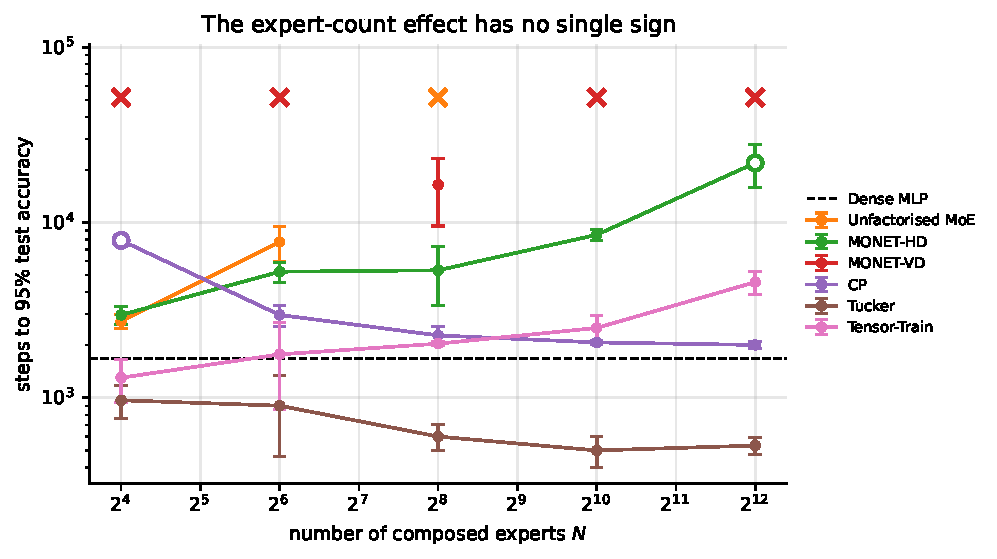
\includegraphics[width=0.85\textwidth]{fig2_grok_vs_experts.pdf}
\caption{Steps to generalisation against the number of composed experts.
Crosses mark configurations where no seed reached the threshold. The curves do
not share a direction: Tucker and CP slope down, Tensor-Train and MONET-HD
slope up, and the unfactorised mixture terminates.}
\label{fig:scaling}
\end{figure}

The claim that more experts is better is therefore not a property of mixtures
of experts. Nor --- and this is where our initial expectation was wrong --- is
it settled by whether the expert tensor is factorised at all. Tensor-Train shares a basis as thoroughly as Tucker does, and keeps it as clean at the two middle expert counts
(Table~\ref{tab:basis-scaling}), yet its grokking step rises with scale while
Tucker's falls. What the results establish is weaker and more specific: the
sign of the effect is a property of the particular factorisation, and a claim
of the form ``more experts is better'' has to be made one architecture at a
time.

\subsection{What survives scaling is the basis, not the router}

The task supplies an independent view of the same models: since the
generalising algorithm must represent operands through Fourier frequencies, we
can ask which frequencies each layer uses, and how that changes as experts are
added.

Figure~\ref{fig:spectra} shows the pooled power spectrum of the shared basis at
$N = 256$ for seed $0$. Averaged over three seeds, the dense MLP spreads its
representation almost evenly, using $38.1$ of the $56$ available frequencies;
MONET-HD concentrates on $7.6$; the Tucker layer solves the same task with $1.7$. A layer with $287\,968$ parameters represents the task in a
two-dimensional frequency subspace, while a layer with $34\,113$ parameters
spreads it over nearly forty.

\begin{figure}[ht]
\centering

\includegraphics[width=\textwidth]{fig5_spectra.pdf}
\caption{Pooled Fourier power of the shared basis as a function of the operand,
at $N = 256$, seed $0$. The effective frequency count is the participation ratio
of the pooled spectrum; three-seed means are given in
Table~\ref{tab:basis-scaling}.}
\label{fig:spectra}
\end{figure}

Table~\ref{tab:basis-scaling} tracks this along the expert-count axis, and it
separates the architectures differently from Table~\ref{tab:scaling}. Tucker
and Tensor-Train both hold a narrow, clean basis as the layer grows: Tucker
between $1.5$ and $1.8$ effective frequencies across a $256\times$ range, and
Tensor-Train at $1.1$ and $1.2$ at $N = 256$ and $N = 1024$, with purity above
$0.94$ at those two counts.
CP broadens steadily ($14.1 \to 35.6$) while its purity nonetheless rises, and
the product-key layers deteriorate on both measures at once --- MONET-HD from
purity $0.891$ and $8.5$ frequencies to $0.150$ and $29.3$, MONET-VD from
$0.881$ and $15.9$ to $0.276$ and $53.4$, against a white-noise purity
reference of $0.082$.

\begin{table}[ht]
\centering
\caption{Effective number of frequencies in the shared basis (top) and
norm-weighted spectral purity (bottom), mean over three seeds. The task has
$56$ frequencies in total; random weights score purity $0.082$.}
\label{tab:basis-scaling}
\footnotesize
\begin{tabular}{lrrrrrr}
\toprule
$N$ & Tucker & CP & Tensor-Train & MONET-HD & MONET-VD & Unfactorised \\
\midrule
\multicolumn{7}{l}{\emph{effective frequencies}} \\
   16 & $1.8$ & $14.1$ & $4.1$  & $8.5$  & $15.9$ & $36.4$ \\
   64 & $1.5$ & $19.2$ & $2.9$  & $8.5$  & $14.5$ & $28.4$ \\
  256 & $1.7$ & $21.7$ & $1.1$  & $7.6$  & $15.9$ & $53.6$ \\
 1024 & $1.7$ & $31.9$ & $1.2$  & $15.0$ & $39.8$ & $55.5$ \\
 4096 & $1.6$ & $35.6$ & $18.6$ & $29.3$ & $53.4$ & --- \\
\midrule
\multicolumn{7}{l}{\emph{basis purity}} \\
   16 & $0.865$ & $0.611$ & $0.713$ & $0.891$ & $0.881$ & $0.824$ \\
   64 & $0.940$ & $0.780$ & $0.732$ & $0.811$ & $0.864$ & $0.796$ \\
  256 & $0.914$ & $0.867$ & $0.948$ & $0.691$ & $0.834$ & $0.138$ \\
 1024 & $0.953$ & $0.879$ & $0.963$ & $0.242$ & $0.606$ & $0.091$ \\
 4096 & $0.951$ & $0.906$ & $0.682$ & $0.150$ & $0.276$ & --- \\
\bottomrule
\end{tabular}
\end{table}

Tensor-Train's apparent collapse at $N = 4096$ is an averaging artefact worth
naming: two of its three seeds hold purity $0.976$ and $0.978$ at $1.11$ and
$1.16$ frequencies, while the third drops to $0.092$ at $53.5$ frequencies ---
and reaches $100\%$ test accuracy anyway, by some route we have not identified.
The mean of $0.682$ describes neither.

The configurations that fail to generalise are the endpoint of this trend
rather than a separate phenomenon. The unfactorised mixture reaches purity
$0.138$ with $53.6$ effective frequencies at $N = 256$, and $0.091$ with $55.5$
of the available $56$ at $N = 1024$: a representation indistinguishable from
noise, produced by a network that fits its training set perfectly.

Across the mixture family, narrower frequency budgets accompany earlier
generalisation, but only loosely: over the $66$ generalising mixture runs the rank correlation between effective frequency count and grokking step is $\rho = 0.50$
(Figure~\ref{fig:freqgrok}). These runs share seeds and their
architectures are nested, so the coefficient summarises the scatter rather than
testing a hypothesis. Two systematic exceptions are visible in it. The dense MLP
uses the widest frequency budget of any model here and still generalises faster
than every product-key variant, and CP broadens its basis steadily with scale
while its grokking step falls. Frequency sparsity is therefore neither necessary
nor sufficient for fast generalisation, and we describe the relationship as a
regularity within the family rather than as a mechanism.

\begin{figure}[ht]
\centering
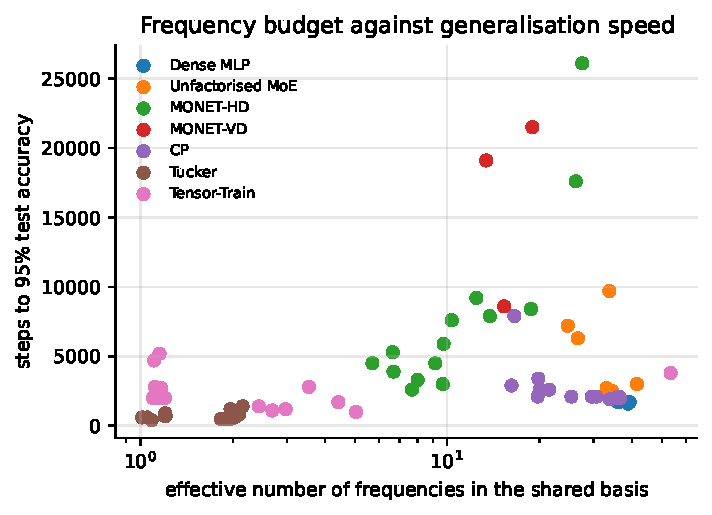
\includegraphics[width=0.8\textwidth]{fig3_freqs_vs_grok.pdf}
\caption{Effective number of frequencies in the shared basis against steps to
generalisation, one point per generalising run. Note the dense MLP (blue), which combines the widest frequency budget with one of the lowest grokking steps.}
\label{fig:freqgrok}
\end{figure}

\paragraph{The router empties out.}
\label{sec:res-router-consequence} Applying the same analysis to the router
gives the most uniform result in this study. Under one-hot inputs the router
logits are a learned lookup table indexed by the operand, so their spectrum is
as directly interpretable as the basis's. Table~\ref{tab:router-scaling} shows
what happens to it.

\begin{table}[ht]
\centering
\caption{Norm-weighted spectral purity of the router keys against expert count,
mean over three seeds. Values at or below the white-noise reference of $0.082$
are in bold. Every architecture ends at or near the floor, though the descent is not monotone for the product-key layers.}
\label{tab:router-scaling}
\footnotesize
\begin{tabular}{lrrrrrr}
\toprule
$N$ & Tucker & CP & Tensor-Train & MONET-HD & MONET-VD & Unfactorised \\
\midrule
   16 & $0.622$ & $0.575$ & $0.607$ & $0.204$ & $0.336$ & $0.552$ \\
   64 & $0.525$ & $0.258$ & $0.458$ & $0.215$ & $0.632$ & $0.570$ \\
  256 & $0.143$ & $0.143$ & $0.177$ & $0.163$ & $0.383$ & $\mathbf{0.089}$ \\
 1024 & $\mathbf{0.072}$ & $\mathbf{0.077}$ & $\mathbf{0.082}$ & $0.192$ & $0.194$ & $\mathbf{0.074}$ \\
 4096 & $\mathbf{0.048}$ & $\mathbf{0.056}$ & $\mathbf{0.059}$ & $0.093$ & $\mathbf{0.076}$ & --- \\
\bottomrule
\end{tabular}
\end{table}

At $N = 16$ every router carries visible structure, scoring between $0.20$ and
$0.62$ against a noise floor of $0.082$. By the largest expert count at which each architecture is run, every router has
fallen to between $0.048$ and $0.093$: at or below the noise floor for five of
the six, and within $14\%$ of it for MONET-HD. The decay holds across all six architectures --- the ones that generalise faster with scale and the ones
that generalise slower, the ones whose bases stay clean and the ones whose
bases decay alongside. Whatever else the choice of factorisation decides, it
does not decide this: adding experts empties the router of interpretable
structure.

The contrast with the basis is sharpest where the basis survives. A Tucker
layer at $N = 4096$ has basis purity $0.951$ and router purity $0.048$: the
computation sits entirely in the shared factors, and the the routing weights carry no more frequency structure than random numbers. Figure~\ref{fig:purity} compares
the two components across architectures, and Figure~\ref{fig:tables} shows them
side by side for a single layer. A complementary measure --- the overlap
between the pooled router spectrum and the pooled basis spectrum, computed on
seed $0$ --- gives the same ordering, with Tucker layers at $0.01$--$0.10$
against $0.46$--$0.78$ for the product-key layers and $0.93$ for the
unfactorised mixture that fails.

\paragraph{The decay is not what empties the router.} Weight decay is applied
to the router keys throughout, which raises the possibility that the collapse
in Table~\ref{tab:router-scaling} is regularisation rather than scale. The
runs that exempt the keys settle it. Exempting them leaves the keys three to
five times larger in root-mean-square magnitude --- $0.557$ against $0.152$
for MONET-HD at $N = 4096$, $0.905$ against $0.336$ at $N = 256$, and $0.270$
against $0.077$ for Tucker at $N = 4096$ --- and does not restore their
spectrum: purity is $0.069$ against $0.093$, $0.119$ against $0.163$, and
$0.045$ against $0.048$ respectively. In every pair the unregularised router
is larger and no better structured. Magnitude and frequency content are
independent here, and it is the second that scaling removes. Note also that
the reference value $0.082$ is the mean purity of random tables of the same
shape rather than a lower bound, so measured values slightly below it are
unremarkable.

\begin{figure}[ht]
\centering
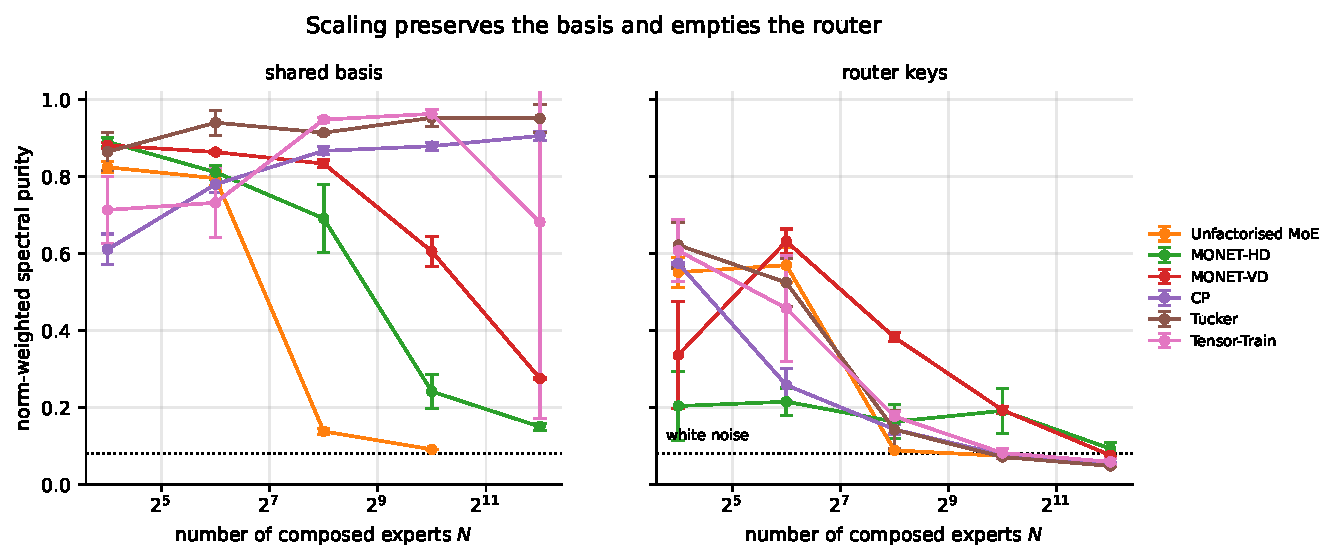
\includegraphics[width=\textwidth]{fig4_purity_basis_vs_router.pdf}
\caption{Norm-weighted spectral purity of the shared expert basis (left)
and of the router keys (right) against expert count, averaged over three
seeds. The dotted line is the purity of a white-noise table ($0.082$).
The dense MLP has neither a basis nor a router and is therefore absent.
The Tucker and CP bases stay clean across the whole sweep, and Tensor-Train's
does except for one seed at $N = 4096$; every router decays to the noise floor.}
\label{fig:purity}
\end{figure}

\begin{figure}[ht]
\centering

\includegraphics[width=\textwidth]{fig6_tables.pdf}
\caption{Shared basis (left) and router keys (right) of a Tucker layer as
functions of the first operand, rows sorted by dominant frequency and
normalised individually, with pooled spectra below. The basis is periodic and
concentrated; the router is not.}
\label{fig:tables}
\end{figure}

This is the observation with the most direct consequence for practice, and the
next section shows how far it reaches. MONET identifies specialised experts by
routing-score skew, and operates at $N = 262\,144$ --- far beyond the point
where, on this task, the router's frequency content has already fallen to
noise. What such a criterion can still recover at that scale, and what it
cannot, is the subject of Section~\ref{sec:res-mixed}.

\subsection{A positive control: what routing scores do recover}
\label{sec:res-mixed}

Every measurement so far is frequency-based, because on single-task modular
addition there is no partition of the input to be specialised towards. The
mixed dataset of Section~\ref{sec:method} supplies one: addition and
multiplication examples over the same operand grid, distinguished by a task
token appended to the input. Here class-based criteria apply, so MONET's own
procedure can be run end to end and checked against ablation --- on a task
where the partition is known exactly. It serves as a positive control: if the
procedure finds nothing here, the negative results above would be evidence
about our measurements rather than about the models.

Both architectures learn the mixed task, and the expert-count trends of
Section~\ref{sec:res-scaling} survive it in weakened form. Tucker generalises
in $1700$, $1800$ and $2100$ steps at $N = 256$, $1024$ and $4096$, so its
improvement with expert count disappears; MONET-HD fails at $N = 256$ and
takes $8800$ and $17300$ steps at the two larger counts, degrading about twice
as steeply as on the single task. Adding a second subtask slows Tucker at every expert count and narrows MONET-HD's window from below.

\paragraph{Procedure.} We follow MONET: a unit is assigned to a subtask when
its mean routing score on that subtask exceeds its score on the other by a
factor of two, and the assignment is then checked by ablation. Two adaptations
are forced by product-key composition. First, a composed expert $(i,j)$ cannot
be ablated individually --- the layer never materialises it, contracting $g^{(1)}$
and $g^{(2)}$ separately --- so we score and ablate the $2Hn$ \emph{factors}
instead, which are the objects the parameters actually correspond to. Second,
ablation sets the factor's routing weight to zero without renormalising the
remainder, so a removed factor contributes nothing, including through its bias
terms. We report accuracy separately on each subtask, and against a control
that ablates the same number of factors chosen uniformly at random, averaged
over twenty draws.

\begin{table}[ht]
\centering
\caption{Applying MONET's specialisation criterion on the mixed task, seed $0$.
``Flagged'' counts the factors assigned to addition, out of $2Hn$. $\Delta$ is
the drop in accuracy on each subtask when those factors are ablated, and
selectivity is $\Delta_{\text{add}} - \Delta_{\text{mul}}$. The control ablates
the same number of factors at random, averaged over twenty draws. MONET-HD at
$N = 256$ did not generalise and is excluded.}
\label{tab:mixed}
\footnotesize
\begin{tabular}{lrrrrrr}
\toprule
 & & \multicolumn{3}{c}{criterion} & \multicolumn{2}{c}{random control} \\
\cmidrule(lr){3-5}\cmidrule(lr){6-7}
Architecture & $N$ & flagged & $\Delta_{\text{add}}$ & selectivity
& $\Delta_{\text{add}}$ & selectivity \\
\midrule
MONET-HD & $1024$ & $33/128$ & $0.981$ & $\mathbf{0.983}$ & $0.601$ & $0.121$ \\
MONET-HD & $4096$ & $51/256$ & $0.965$ & $\mathbf{0.969}$ & $0.269$ & $-0.237$ \\
Tucker   & $256$  & $31/64$  & $0.987$ & $\mathbf{0.987}$ & $0.233$ & $0.211$ \\
Tucker   & $1024$ & $51/128$ & $0.993$ & $\mathbf{0.993}$ & $0.021$ & $-0.058$ \\
Tucker   & $4096$ & $67/256$ & $0.991$ & $\mathbf{0.991}$ & $0.005$ & $0.003$ \\
\bottomrule
\end{tabular}
\end{table}

\paragraph{The criterion passes, and passes at every scale.} Table~\ref{tab:mixed}
is unambiguous. Ablating the factors that routing scores assign to addition
removes addition entirely --- accuracy falls by $0.97$ to $0.99$ --- and leaves
multiplication untouched, with $\Delta_{\text{mul}}$ between $-0.004$ and
$0.000$ in every configuration. The random control removes the same number of
factors and damages both subtasks indiscriminately, with selectivity ranging
from $0.21$ down to $-0.24$. The effect does not weaken with expert count: at
$N = 4096$, where the same routers score $0.048$ and $0.093$ on spectral
purity against a white-noise floor of $0.082$, selectivity is still $0.99$.

One feature of the table is a check on the procedure rather than a result.
No factor on the first side of the router is ever flagged. With $d_{\text{in}} = 228$ the router's split puts coordinates $0$--$113$ on the
first side --- the whole of $\mathrm{onehot}(a)$ together with the single
coordinate for $b = 0$ --- and everything else, including both task-token
coordinates, on the second, so the first side cannot
see which subtask an example belongs to and correctly reports no
specialisation. The method is not producing noise; it finds structure exactly
where structure exists.

\paragraph{What this does to the router result.} The two halves of the study
now say something sharper than either does alone. The same routers that have
lost their frequency content by $N = 4096$ still carry the subtask partition
perfectly, and routing-score attribution recovers it with near-perfect
selectivity. A router is therefore not emptied by scale in any absolute sense.
What it loses is the structure that implements the algorithm; what it keeps is
the structure the input already announces.

This is a worse position for routing-score interpretability than a simple
failure would be. The criterion and the ablation agree here because both read
the same partition, so their agreement validates the partition rather than the
mechanism, and a method that checks one against the other cannot tell the
difference. MONET's domains --- Python, chemistry, toxic text --- are partitions
of the first kind, largely readable from the tokens themselves. A routing-based
criterion will find experts that track them, the ablation check will confirm
it, and none of that is evidence about how the model computes anything.

\subsection{Ablations}
\label{sec:res-ablations}

Four ablations at seed $0$ --- router-key decay at both $N = 256$ and
$N = 4096$, the other three at $N = 256$ --- isolate mechanisms that
would otherwise remain conjectural. Results are in Table~\ref{tab:ablations};
the baseline column repeats the corresponding main-grid run for the same seed.

\begin{table}[ht]
\centering
\caption{Ablations. ``fail'' gives the final test accuracy in parentheses. The
baseline configuration is a natural input split, $\lambda = 10^{-3}$, router
keys decayed, $80\%$ training fraction. Rows marked $\dagger$ are over three
seeds, reported as mean $\pm$ sd; all other entries are seed $0$.}
\label{tab:ablations}
\footnotesize
\begin{tabular}{llrrr}
\toprule
Ablation & Architecture & \multicolumn{3}{c}{Grokking step} \\
\midrule
\emph{Router-key decay} & & decayed & exempt & \\
& Tucker, $N{=}256$       & $600$  & $600$ & \\
& Tucker, $N{=}4096$      & $600$  & $600$ & \\
& MONET-HD, $N{=}256^\dagger$  & $5333 \pm 1986$ & $5800 \pm 929$ & \\
& MONET-HD, $N{=}4096^\dagger$ & $21850 \pm 6010$\,[2/3] & fail $(0.006$--$0.090)$ & \\
& Unfactorised, $N{=}256$ & fail $(0.000)$ & fail $(0.007)$ & \\
\midrule
\emph{Router input split} & & natural & interleaved & random \\
& Tucker, $N{=}256$   & $600$  & $5100$ & $1700$ \\
& MONET-HD, $N{=}256$ & $7600$ & fail $(0.823)$ & fail $(0.822)$ \\
\midrule
\emph{Auxiliary loss $\lambda$} & & $0$ & $10^{-3}$ & $10^{-2}$ \\
& Tucker, $N{=}256$   & $500$  & $600$  & $800$ \\
& MONET-HD, $N{=}256$ & $6500$ & $7600$ & $3000$ \\
\midrule
\emph{Training fraction} & & $0.4$ & $0.6$ & $0.8$ \\
& Tucker, $N{=}256$   & $6300$ & $800$  & $600$ \\
& MONET-HD, $N{=}256$ & fail $(0.004)$ & $8200$ & $7600$ \\
\bottomrule
\end{tabular}
\end{table}

\paragraph{Router-key decay matters where memorisation is cheap.} Under one-hot
inputs the router keys form a table of $8nP$ parameters addressed directly by the operand value --- $14\,464$ of them at $N = 256$ and $57\,856$ at $N = 4096$.
Exempting them from weight decay, as is conventional for router parameters,
leaves that table unregularised. At the $80\%$ training fraction used throughout, the cost appears only where
the table is largest, and it is decisive there. Over three seeds at
$N = 4096$, exempting the keys costs generalisation on every one, with final
test accuracies of $0.006$, $0.013$ and $0.090$, against two successes in
three for the decayed setting; at $N = 256$ the two settings are
indistinguishable, $5333 \pm 1986$ against $5800 \pm 929$. For Tucker the ablation makes no difference at either expert count.

The effect is far larger when data is scarcer. During protocol selection
(Section~\ref{sec:protocol}) we compared the two settings at a $50\%$ training
fraction with $N = 256$: with the keys exempt, test accuracy was $0.006$; with
the keys decayed, the layer grokked at step $15\,000$ and reached $0.977$.
Both the data fraction and the expert count control how attractive the
memorisation shortcut is, and the convention of exempting router parameters is
safe only while it stays unattractive --- which is not something one can assume
without checking.

\paragraph{The natural input split matters, and unequally.} When the router's
two halves are the two operands, the factorisation of the router matches the
factorisation of the task. Permuting the input destroys that alignment.
MONET-HD then fails under both permutations, reaching only $0.82$ test
accuracy; Tucker survives both, slowed by $8.5\times$ under interleaving and
$2.8\times$ under a random permutation. Part of the advantage we report is
therefore due to structural alignment rather than to factorisation as such, and
the effect is large enough to state plainly rather than file under caveats. It
is also informative that the two architectures depend on it to different
degrees: alignment is what lets the product-key layer work here at all, while
for Tucker it is an accelerant. We have no account of why interleaving costs Tucker more than a random
permutation does.

\paragraph{The auxiliary losses do little.} MONET's uniformity and ambiguity
terms move Tucker's grokking step from $500$ at $\lambda = 0$ to $600$ and
$800$ as $\lambda$ rises --- a mild cost. For MONET-HD the three values give $6500$, $7600$ and $3000$: not monotone, and
the drop at $\lambda = 10^{-2}$ is $2.3$ standard deviations of that
configuration's seed spread, which a single seed cannot separate from noise. We
record it as unresolved rather than as an effect. Since these terms were calibrated for language
modelling, where cross-entropy never approaches zero, their near-neutrality on
an algorithmic task is unsurprising. What is worth recording is that they are
not a prerequisite for anything we observe: the frequency structure and the
router decay both appear at $\lambda = 0$.

\paragraph{Data efficiency follows the same ordering.} At a $40\%$ training
fraction Tucker still generalises, in $6300$ steps, while MONET-HD does not
generalise at all ($0.004$ test accuracy). At $60\%$ Tucker takes $800$ steps
and MONET-HD $8200$. The gap widens as data is withdrawn, which is what one
expects if the shared basis acts as a prior rather than as extra capacity.

\subsection{The rank effect has no single sign either}
\label{sec:res-rank}

The architectures that improve with expert count share a property: their
capacity along the expert modes grows with $n$. Our Tucker layer uses an
expert-mode rank of $\min(32, n)$ and CP projects onto $n$ columns, so both
widen as experts are added. Tensor-Train does not: its two expert-mode cores
are joined through a bond whose rank we held fixed at $16$ across the whole
sweep. A natural account of why Tensor-Train degrades while Tucker improves is
therefore that its added experts cannot refine the computation and can only be
used to fit the training set. Two experiments test that account, and they
disagree with each other.

\begin{table}[ht]
\centering
\caption{Rank sweep, seed $0$. Grokking step, with parameter count in
parentheses for the Tensor-Train rows. ``fail'' gives the final test accuracy.
The Tucker row freezes the expert-mode rank at $4$ so that it cannot grow with
$n$; the main-grid Tucker layer, whose rank is $\min(32, n)$, generalises in
$600$ steps at both $N = 256$ and $N = 4096$ on this seed.}
\label{tab:rank}
\footnotesize
\begin{tabular}{lccc}
\toprule
 & $N = 256$ & $N = 1024$ & $N = 4096$ \\
\midrule
\multicolumn{4}{l}{\emph{Tensor-Train}} \\
rank $8$  & $1400$ ($31$K)           & $2800$ ($47$K)            & $4300$ ($78$K) \\
rank $16$ & $2100$ ($78$K)           & $2000$ ($97$K)            & $4700$ ($135$K) \\
rank $32$ & fail $(0.866)$ ($266$K)  & $5600$ ($298$K)           & $7100$ ($360$K) \\
rank $64$ & fail $(0.022)$ ($1014$K) & fail $(0.187)$ ($1095$K)  & $16\,300$ ($1257$K) \\
\midrule
\multicolumn{4}{l}{\emph{Tucker}} \\
rank $4$, frozen & fail $(0.301)$ & $1800$ & $2400$ \\
\bottomrule
\end{tabular}
\end{table}

\paragraph{Giving Tensor-Train more rank makes it worse, not better.} The
prediction fails on both counts. The grokking step still rises with expert
count at every rank tested --- from $1400$ to $4300$ at rank $8$, from $2100$
to $4700$ at rank $16$, from $5600$ to $7100$ at rank $32$ --- so the upward
trend is not an artefact of the bottleneck we happened to fix. And raising the
rank does not help at any expert count. It helps at no expert count but one --- rank $16$ beats rank $8$ at $N = 1024$,
$2000$ steps against $2800$ --- and beyond rank $16$ it opens a failure region that widens as the rank grows: at rank $64$ and
$N = 256$ a layer holding over a million parameters fits the training set
perfectly and reaches test accuracy $0.022$.

CP separates two things the rest of this section treats together. Its units
become purer as experts are added --- purity rises from $0.611$ to $0.906$ ---
while the layer as a whole spreads over more frequencies, from $14.1$ to
$35.6$. By the per-unit criterion CP is the most monosemantic layer here; by
the layer-level criterion it is among the least sparse. Monosemanticity of
units and sparsity of the layer's frequency budget are therefore not the same
property, and the claim that a shared basis acts as a sparsity prior holds for
Tucker and Tensor-Train but not for CP.

What the sweep does track is parameter count. Rank enters the Tensor-Train
parameter count multiplicatively, so rank $64$ costs between $16$ and $33$
times rank $8$ at the same expert count, and the configurations that fail are
those where that cost is largest relative to the number of experts it buys.
This is the signature of the unfactorised mixture, which generalises at
$N = 64$ with $189\,000$ parameters and fails at $N = 256$ with $740\,000$. We
record it as a description rather than a mechanism: it orders the Tensor-Train
family and does not transfer across architectures, since a Tucker layer with
$288\,000$ parameters generalises at $N = 256$ in $600$ steps.

\paragraph{Freezing Tucker's rank removes its improvement.} The converse test
holds the Tucker expert-mode rank at $4$ so that it cannot grow with $n$. The
improvement disappears. At $N = 256$ the layer fails --- not by memorising but
by failing to fit at all, reaching training accuracy $0.432$ --- and beyond
that it degrades from $1800$ to $2400$ steps as experts are added, where the
unfrozen layer stays near $600$ throughout. On the Tucker side, then, growing
rank is exactly what converts added experts into faster generalisation.

Taken together the two experiments say something narrower than the account they
were built to test, and something that echoes
Section~\ref{sec:res-scaling}: rank growth is what lets Tucker benefit from
added experts, and the absence of rank growth is not what stops Tensor-Train.
The sign of the rank effect, like the sign of the expert-count effect, is a
property of the particular factorisation.

\paragraph{A reproducible anomaly.} Section~\ref{sec:res-stability} reports one
main-grid Tensor-Train seed that reaches perfect test accuracy at $N = 4096$
with a basis indistinguishable from noise. The rank sweep reproduces it on
demand: at rank $32$ and $N = 4096$ the layer generalises in $7100$ steps with
basis purity $0.081$ and $55.9$ effective frequencies, and at rank $64$ and
$N = 4096$ it reaches $0.998$ test accuracy with purity $0.082$. The effect is
systematic at high rank rather than a rare initialisation. We read it as a
limitation of the measurement rather than of the model: what we extract as the
shared basis of a Tensor-Train layer is its input core, and at high rank the
operand representation evidently moves elsewhere along the chain. The
Tensor-Train entries of Table~\ref{tab:basis-scaling} should be read with that
in mind.

One positive result comes out of the same runs. Tucker with rank $4$ reaches
basis purity $0.995$ and $0.993$ at $1.01$ effective frequencies for
$N = 1024$ and $N = 4096$ --- the cleanest representations anywhere in this
study, produced by layers of $31\,000$ and $60\,000$ parameters. A rank-four
expert basis solves modular addition with what is essentially a single
frequency.

\subsection{How much of the Tucker core is used}
\label{sec:res-comp}

Two facts established above point at the same object. Tucker generalises
fastest of the layers we compare, and it is also the multilinear layer whose
parameter count still rises steeply with expert count
(Table~\ref{tab:params}). Both properties live in the core, which is the only
place where the two expert modes interact. We therefore constrain that
interaction and ask how much of it the task actually uses.

Write the expert-mode slice of the core at rank $r$,
\begin{equation}
\mathcal{Z}[p, q, a, c]
  \;=\; \sum_{s=1}^{r} W[p, q, s]\, C^{(a)}[s, a]\, C^{(b)}[s, c],
\end{equation}
so that $r = 1$ makes the layer's dependence on the two routing vectors
separable, and the dense core is recovered at $r = R_a^2$, which is $256$ at
$N = 256$ and $1024$ above it. The initialisation is scaled so that the
implied core entries have the same variance at every $r$, and the rearranged
forward pass is verified against the naive sum over all $n^2$ composed experts
in the same way as the other layers.

One thing this family does \emph{not} do should be said before the numbers.
At $r = 1$ it does not reduce to product-key composition. MONET's layers apply
a nonlinearity between the two factors and are therefore not multilinear,
whereas a rank-one multilinear coupling is a strictly weaker object: a
trilinear form of rank one. The sweep varies how much the two expert modes may
interact inside a multilinear layer; it does not interpolate towards MONET.

\begin{table}[ht]
\centering
\caption{Composition-rank sweep, seed $0$. Grokking step, with parameter count
in parentheses. ``fail'' gives the final test accuracy; at ranks $1$ and $2$
the layer does not fit the training set either, reaching training accuracy
$0.23$ and $0.53$ at $N = 256$. The dense row repeats the three-seed means of
Table~\ref{tab:scaling} and the parameter counts of Table~\ref{tab:params}. The row marked $\dagger$ is over three seeds; all other rows are seed $0$.}
\label{tab:comp}
\footnotesize
\begin{tabular}{lccc}
\toprule
coupling rank & $N = 256$ & $N = 1024$ & $N = 4096$ \\
\midrule
$1$     & fail $(0.005)$ & fail $(0.007)$ & fail $(0.035)$ \\
$2$     & fail $(0.016)$ & fail $(0.029)$ & fail $(0.025)$ \\
$4$     & fail $(0.671)$ & fail $(0.475)$ & $1200$ \quad ($77$K) \\
$8$     & $800$ \quad ($34$K) & $900$ \quad ($51$K) & $800$ \quad ($82$K) \\
$16$    & $700$ \quad ($43$K) & $500$ \quad ($59$K) & $500$ \quad ($90$K) \\
$32$    & $600$ \quad ($60$K) & $500$ \quad ($77$K) & $500$ \quad ($108$K) \\
\midrule
dense$^\dagger$ & $600$ \quad ($288$K) & $500$ \quad ($1090$K) & $533$ \quad ($1121$K) \\
\bottomrule
\end{tabular}
\end{table}

\paragraph{A threshold, then nothing.} Table~\ref{tab:comp} shows a sharp
transition rather than a gradual trade-off. At ranks $1$ and $2$ the layer cannot fit the training set, let alone
generalise. That much is closer to a structural fact than to a measurement: at
$r = 1$ the layer computes a sum over heads of a linear map of the input times
a scalar function of $a$ times a scalar function of $b$, and and modular addition does not lie in that family: with $r = 1$ the
head-dependent factors enter only as scalars, so the layer computes
$s(a, b)\,\bigl(v_a(a) + v_b(b)\bigr)$ for a scalar $s$ and vectors
$v_a, v_b \in \mathbb{R}^{P}$, and the class that maximises such an expression
cannot depend on $a$ and $b$ jointly in the way $(a + b) \bmod P$ requires. What the table adds is where the threshold sits
and what happens above it. At rank $4$ it fits but
generalises only at the largest expert count. From rank $8$ upward it
generalises everywhere, and from rank $16$ it is indistinguishable from the
dense core: $700$, $500$ and $500$ steps against $600$, $500$ and $533$, all
within the seed spread that Section~\ref{sec:res-stability} reports for this
architecture.

\paragraph{The dense core is over-provisioned by an order of magnitude.} The
rank-$32$ layer at $N = 4096$ holds $107\,616$ parameters against $1\,121\,376$
for the dense core --- a factor of $10.4$ --- and generalises in $500$ steps
against $533 \pm 58$. Measured across the sweep, the parameter growth from
$N = 256$ to $N = 4096$ falls from $3.89\times$ to $1.81\times$. A coupling of rank $32$ out of a possible $1024$ is all the task uses, and rank
$8$ suffices at a cost of between a third and four fifths more steps.

This bears directly on the objection MONET raises against multilinear expert
layers (Section~\ref{sec:related}), that their parameter counts grow too
quickly with expert count to compete with product-key composition. On this
task the growth is real but almost entirely unused: it sits in core entries
that carry no signal, and constraining the coupling removes most of it at no
measurable cost in generalisation speed. The comparison between the two
families is therefore not settled by the parameter counts of the layers as
published.

\paragraph{Experts partly substitute for coupling.} At rank $4$ the layer
fails at $N = 256$ and $N = 1024$ and generalises at $N = 4096$. Where the
coupling is too poor to express the task at one expert count, adding experts
can recover it --- another instance of the window of Section~\ref{sec:res-scaling},
now with one of its two coordinates under direct control.

\subsection{Stability under reinitialisation}
\label{sec:res-stability}

A final observation emerges only with multiple seeds. At $N = 256$ the standard
deviation of the grokking step is $100$ steps for Tucker, $58$ for
Tensor-Train and the dense MLP, $289$ for CP, but $1986$ for MONET-HD and
$6861$ for MONET-VD, whose individual seeds grok at $8600$, $19100$ and
$21500$ --- a spread wider than the entire range separating the other six
architectures.

Instability also appears at the largest expert counts in architectures that are
otherwise stable, and not only in the grokking step: the Tensor-Train seed
described above, which collapses to a noise-like basis at $N = 4096$ while
still reaching perfect accuracy, has no counterpart among its siblings.
Averages at $N = 4096$ should be read with this in mind.

Product-key composition is thus not only slower but far less predictable, and a
single-seed comparison of these architectures would be seriously misleading in
either direction. This is consistent with the weak universality reported for
group-composition tasks by \citet{chughtai2023universality}, and it is why the
claims in this section are stated over seeds rather than over runs.
\section{Discussion}
\label{sec:discussion}

\subsection{What the results do and do not show}

We began with the expectation that the architectures would order themselves by
how much of the expert parameterisation is shared: independent experts at one
end, product-key composition in the middle, multilinear factorisations at the
other, with generalisation improving monotonically along that axis. The two
endpoints behave as expected. The middle does not survive contact with the
data, because Tensor-Train sits firmly at the shared end and scales like the
product-key layers rather than like Tucker.

What remains is a weaker and more useful statement. Every architecture we
tested has a window of expert counts in which it generalises, and the
factorisation determines where that window sits and how wide it is.
Independent experts have the narrowest: they work at $N = 16$ and $N = 64$ and
fail completely at $N = 256$. CP has a window with a visible lower edge --- at
$N = 16$ two seeds in three fail --- and no upper edge within our range.
Tucker's window covers the entire range, with its best performance at the top.
MONET-HD degrades steadily and begins to fail at $N = 4096$. Whether adding
experts helps is therefore a question about where a given architecture
currently sits in its own window, not a question about mixtures of experts.

Two mechanisms plausibly set the two edges, and the ablations let us say
something about each rather than speculate.

The upper edge is at least partly the router. Under one-hot inputs the router
keys form a table of $8nP$ parameters addressed directly by the operand, and it
grows linearly in $n$. Section~\ref{sec:res-ablations} shows this is a real
memorisation channel and not a hypothetical one: at $N = 4096$, exempting those
keys from weight decay costs MONET-HD generalisation outright, and at a $50\%$
training fraction the same exemption is the difference between $0.006$ and
$0.977$ test accuracy. The channel is harmless while memorisation is
unattractive and becomes decisive when it is not, which is exactly the regime
large expert counts create.

The lower edge is partly rank starvation in the expert modes, but only on one
side. Our Tucker layer uses an expert-mode rank of $\min(32, n)$, so at $n = 4$
the routing coefficients are compressed into a four-dimensional space and the
experts are nearly indistinguishable; CP at $n = 4$ projects a rank-$128$
factor onto four columns. Both architectures are at their worst there, and both
improve as $n$ rises to meet their rank. Section~\ref{sec:res-rank} tests this
directly by freezing the Tucker rank at $4$, and the improvement disappears:
the layer stops fitting at all at $N = 256$ and then slows from $1800$ to
$2400$ steps as experts are added, where the unfrozen layer stays near $600$.

The same account predicted that Tensor-Train, whose expert-mode bond we held at
rank $16$ throughout the sweep, would be rescued by letting that rank grow. It
is not. Raising the rank leaves the upward trend in expert count intact at
every value tested and makes the layer worse at every expert count, opening a
failure region that widens with rank until, at rank $64$ and $N = 256$, a
layer of over a million parameters memorises the training set and reaches
$0.022$ test accuracy. We state the prediction and its failure because the
failure is the more informative half. The sign of the rank effect turns out to
be a property of the particular factorisation, exactly as the sign of the
expert-count effect is, and our search for a single quantity that sets the
direction for every architecture has now come up empty twice. The upper-edge
account stands as it is, since the router ablation supports it directly.

\subsection{Consequences for routing-score interpretability}

The router result is the one that does not depend on which architecture is
better. Across all six mixture layers, and regardless of whether that layer
generalises sooner or later with scale, the spectral purity of the router keys falls as experts are added, reaching the white-noise floor at the largest expert count each is run at. In
the same layers where the shared basis stays clean --- Tucker at purity
$0.951$, Tensor-Train at $0.976$ on the seeds that behave --- the router has
fallen to $0.048$ and $0.059$. The computation and the routing end up in
different places, and the gap widens with scale.

The obvious reading of that --- routing scores stop being informative at scale
--- is wrong, and Section~\ref{sec:res-mixed} shows why. On the mixed task the
same routers at the same expert count support MONET's criterion perfectly:
factors assigned to a subtask by routing-score skew are exactly the factors
whose removal destroys that subtask and spares the other, with selectivity
$0.99$ at $N = 4096$. A router that scores at the white-noise floor on
frequency content is still a flawless detector of which subtask it is looking
at.

The correct statement is therefore about what kind of structure survives.
Routing scores recover partitions that the input already carries, and miss the
structure that performs the computation; scaling drains the second and leaves
the first. This is a more uncomfortable position for routing-based
interpretability than plain uninformativeness would be. A method that
identifies experts by routing-score skew and validates the identification by
ablation is checking one reading of the partition against another, so the two
agree by construction, and the agreement certifies nothing about mechanism.
Nothing inside such a method signals which of the two situations it is in.
MONET's domains --- Python, chemistry, toxic text --- are partitions of the
kind that is largely readable from the tokens, which is precisely the regime
where the criterion will look most convincing and mean least.

We would not extrapolate to language models on the strength of one algorithmic
testbed. What the testbed establishes is that the dissociation can occur, that
the frequency half of it strengthens with scale, and that the standard
validation procedure cannot detect it. Testing for it in a language model does
not require Fourier analysis: it requires a task where the mechanism is known
independently of the domain label, so that routing-score attribution can be
scored against something other than the partition it was derived from.

\subsection{Limitations}
\label{sec:limitations}

\paragraph{Structural alignment.} The multilinear layers compute a product of a
factor depending on $a$ and a factor depending on $b$, and the Fourier solution
of modular addition has exactly that form. The architecture is aligned with the
target function in a way specific to this task. We measured the size of that
advantage rather than leaving it as a caveat: permuting the router's input so
that its halves are no longer the two operands slows Tucker by $8.5\times$
under interleaving and $2.8\times$ under a random permutation, and makes
MONET-HD fail entirely. Alignment therefore accounts for a substantial part of
what we report, and the correct statement of the result is that a decomposition
whose structure matches the structure of the task both generalises sooner and
yields a sparser representation in the task's own basis. Establishing anything
more general requires tasks whose solutions are not multiplicative in the
operands.

\paragraph{One task, one modulus.} All results are for $c = (a+b) \bmod 113$
with one-hot inputs and a single hidden layer. Nothing here demonstrates
transfer to language models, which is where MONET operates and where the
monosemanticity claims we examine were made.

\paragraph{Mechanisms are partly tested.} The router-table account of the upper
edge is supported by the ablations, and the rank account of the lower edge has
now been tested on both sides: confirmed for Tucker, refuted for Tensor-Train,
which leaves the Tensor-Train trend without a mechanism.

\paragraph{Ranks and widths are not matched.} CP is given rank $128$, Tucker
$32$, Tensor-Train $16$, and every layer an expert dimension of $8$. These were
chosen to put the architectures in a comparable parameter range rather than by
any principle, and Section~\ref{sec:res-comp} shows that at least one of them
is an order of magnitude from binding. Differences we attribute to the
structure of a decomposition may therefore be partly differences in how
generously each one happens to be provisioned.

\paragraph{One training regime, selected on one architecture.} The protocol of
Section~\ref{sec:protocol} was fixed by a sweep over the dense MLP and then
applied unchanged to every Mixture-of-Experts layer, although
Section~\ref{sec:protocol} itself observes that the grokking band depends on
the architecture. Learning rate, weight decay, the Adam betas and the
auxiliary weight are therefore tuned for one member of the comparison and
inherited by the other six. This is the largest confound in the study. It
bears most heavily on the configurations that fail: MONET-VD fails at four of
five expert counts and generalises at one, and we cannot distinguish an
architectural property from a regime that suits it badly at the other four.

\paragraph{Weight decay is not the same regulariser in every format.} An $L_2$
penalty applied to CP factors induces a penalty on the reconstructed tensor
close to a nuclear norm; applied to a Tucker core and its factors it induces a
different one; applied to a chain of Tensor-Train cores, a third. Holding the
coefficient at $1.0$ across architectures therefore does not hold the
regularisation fixed --- it varies it in a way determined by the very
factorisation we are trying to isolate. This is a plausible partial account of
why the sign of the expert-count effect differs between formats, and it is not
one our experiments can separate from the structural account we give.

\paragraph{Seeds are uneven across experiments.} Section~\ref{sec:method}
states that three seeds are used for every configuration carrying a claim, and
that holds for the main grid and for the router-key decay ablation. It does
not hold for the remaining ablations, the rank sweeps of
Sections~\ref{sec:res-rank} and~\ref{sec:res-comp}, or the mixed-task control,
all of which are seed $0$. For architectures whose seed spread reaches $6861$
steps, single-seed differences below roughly $2000$ steps should be read as
suggestive.

\paragraph{Degradation factors are lower bounds.} Failed runs are excluded
from the averages rather than assigned the step budget, so a statement such as
``MONET-HD degrades by $7.4\times$'' compares the seeds that survived at each
expert count. Where some seeds fail at the larger count, as at $N = 4096$, the
true degradation is worse than the figure given.

\paragraph{Frequency sparsity is a correlate, not a law.} Within the mixture
family, narrower frequency budgets accompany earlier generalisation, but the
dense MLP violates the trend, using $38.1$ effective frequencies and still
generalising faster than every product-key variant. CP broadens its basis
steadily with scale while its grokking step falls. We therefore describe the
relationship as a regularity within the family rather than as a mechanism.

\paragraph{Unexplained cases.} MONET-VD fails at $N = 16$, $64$, $1024$ and
$4096$ and generalises only at $N = 256$; we report this rather than omit it,
and have no account of it. One Tensor-Train seed at $N = 4096$ reaches perfect test accuracy with a basis
indistinguishable from noise; Section~\ref{sec:res-rank} shows this is
systematic at high rank and is most likely a limitation of how we extract the
basis for this format rather than a property of the model.

\paragraph{Fixed data partition and single-seed ablations.} Seeds vary
initialisation only; the train/test split is held fixed, which isolates
initialisation variance but says nothing about sensitivity to which pairs are
withheld. Most of the ablations use one seed, so the differences reported there are not
protected against the seed variance that Section~\ref{sec:res-stability}
documents for the product-key layers in particular; the router-key decay ablation, on which the upper-edge account rests, is the exception and is run on three.

The mixed-task control of Section~\ref{sec:res-mixed} is likewise seed $0$
only, and ablates router factors rather than composed experts, which
product-key composition does not allow to be removed individually.

\subsection{Future work}
\label{sec:future}

The most direct continuation is the decomposition this study did not train.
Tucker performs best here, but its core grows as $\prod_n R_n$, which is why
its parameter count still rises steeply with expert count in
Table~\ref{tab:params} while CP's and Tensor-Train's do not.
Section~\ref{sec:res-comp} shows that most of that growth is unused, which
makes the hierarchical Tucker format \citep{grasedyck2010hierarchical} a way of
removing it by construction rather than by a rank constraint imposed after the
fact: instead of one dense core, the modes are arranged on a binary tree with a
small transfer tensor at each internal node, giving parameter count linear
rather than exponential in the order while retaining the pairwise mode
interactions that CP lacks.

Applied to an expert layer the construction is natural. Factor the expert index
into $L$ binary modes, $N = 2^L$, and place them at the leaves of a balanced
tree. Routing then becomes hierarchical: a token descends the tree, making one
binary decision per level, and selects an expert in $O(\log N)$ rather than
$O(\sqrt{N})$ decisions. Two properties follow that bear on the questions
raised here. The internal nodes carry representations at intermediate levels of
granularity, so the hierarchy itself becomes an object of interpretation ---
coarse concepts near the root, fine ones near the leaves --- rather than only
the leaves, as in a flat expert set. And the transfer tensors are shared across
all experts beneath a node, so sharing is graded by depth rather than fixed by
a single global choice. Given that our results turn on where each
architecture's usable window of expert counts sits, an architecture with a
tunable sharing gradient is the natural instrument for asking what sets the
edges of that window.

Three further directions follow from the limitations. Identifying what does set the direction for Tensor-Train, now that rank is
ruled out, together with an extraction of the operand representation from the
whole core chain rather than from the input core alone. Tasks whose solutions are not
multiplicative in the operands, which would separate the effect of
factorisation from the effect of structural alignment. And the same
router-versus-mechanism comparison on a small language model, where the shared
basis cannot be Fourier-analysed but routing-score attribution and ablation can
still be set against each other.

\section{Conclusion}

We asked whether scaling the number of experts in a Mixture-of-Experts layer
makes it more interpretable, on a task where the answer can be checked rather
than illustrated. It does not, and the reason is more specific than we
expected. Adding experts brings generalisation forward for some factorisations
of the expert tensor, pushes it back for others, and destroys it for
independent experts --- with Tensor-Train and Tucker landing on opposite sides
despite sharing their parameters equally thoroughly. Each architecture has a
window of expert counts in which it works, and the factorisation sets where
that window lies.

One result holds across all of them. As experts are added, the router's
frequency content decays to noise in every mixture architecture we tested,
while the shared basis of the best-scaling ones stays clean --- so the
computation and the routing end up in different places, and the gap widens
with scale. The router does not go blank: on a control task whose subtask is
signalled in the input, routing-score attribution still identifies the
responsible factors perfectly at the largest expert count we tested. What it
recovers is the partition the input already carries; what it misses is the
structure that performs the computation, and from inside the method the two
look the same. Whether that dissociation holds in language models is the
question this testbed was built to make askable.

\newpage
\printbibliography[heading=bibintoc]

\newpage
\appendix
\section{Rearranged Forward Passes}
\label{app:forward}

A factorised expert layer is useful only if it is never materialised. Written
naively, a product-key layer sums over $H n^2$ terms per token; written
correctly, the same quantity costs $O(H n)$. The rearrangement is where
implementation errors hide, because a wrong contraction still trains and still
drives the loss down --- it simply computes a different function than the one
described. This appendix records the derivations and the check that was run
against them.

Throughout, $\gvec^{(1)}_{hi}$ and $\gvec^{(2)}_{hj}$ are the routing weights
of Equation~\eqref{eq:product-key}, $x \in \R^{d_{\mathrm{in}}}$ is the input,
and indices $i,j$ run over the $n$ factors per side.

\subsection{Horizontal decomposition}

With $E_{ij}$ as in Equation~\eqref{eq:hd}, the layer output is
\begin{equation}
  y = \sum_{h} \sum_{i} \sum_{j}
      \gvec^{(1)}_{hi}\gvec^{(2)}_{hj}
      \Big( V_j\, \sigma(U_i x + b^{(1)}_i) + b^{(2)}_j \Big).
\end{equation}
Write $z_i = \sigma(U_i x + b^{(1)}_i) \in \R^{m}$, computed once for each of
the $n$ bottom factors. The first term factors as
\begin{equation}
  \sum_{h}\sum_{j} \gvec^{(2)}_{hj} V_j
  \underbrace{\sum_{i} \gvec^{(1)}_{hi} z_i}_{t_h \in \R^{m}}
  \;=\;
  \sum_{j} V_j \underbrace{\sum_{h} \gvec^{(2)}_{hj} t_h}_{u_j \in \R^{m}},
\end{equation}
so the bottom factors are collapsed per head into $t_h$ and redistributed to
the top factors as $u_j$, and the $n^2$ expert combinations never appear. The
bias term collapses to $\sum_j c_j b^{(2)}_j$ with $c_j = \sum_h
\gvec^{(2)}_{hj}\sum_i \gvec^{(1)}_{hi}$; when the routing weights are
normalised the inner sum is one, recovering the form given by
\citet{park2025monet}. We implement the general form, which is correct whether
or not normalisation holds.

\subsection{Vertical decomposition}

Here expert $(i,j)$ produces the first half of the output from factor $i$ and
the second half from factor $j$, each acting on both halves of the hidden
state. With $p^{(1)}_i = \sigma(U^{(1)}_i x + b^{(1)}_i)$ and $p^{(2)}_j =
\sigma(U^{(2)}_j x + b^{(2)}_j)$, the two output blocks are
\begin{align}
  y_{\mathrm{top}} &= \sum_i A_i V^{11}_i p^{(1)}_i
                    + \sum_i V^{12}_i \sum_h \gvec^{(1)}_{hi}
                      \sum_j \gvec^{(2)}_{hj} p^{(2)}_j
                    + \sum_i A_i b^{12}_i, \\
  y_{\mathrm{bot}} &= \sum_j B_j V^{22}_j p^{(2)}_j
                    + \sum_j V^{21}_j \sum_h \gvec^{(2)}_{hj}
                      \sum_i \gvec^{(1)}_{hi} p^{(1)}_i
                    + \sum_j B_j b^{22}_j,
\end{align}
where $A_i = \sum_h \gvec^{(1)}_{hi}\sum_j \gvec^{(2)}_{hj}$ and $B_j = \sum_h
\gvec^{(2)}_{hj}\sum_i \gvec^{(1)}_{hi}$. The cross terms are the reason this
variant is more expensive than the horizontal one despite an identical
parameter count: each requires an extra pass through the head index. Since
$P = 113$ is odd, the output is split into blocks of $57$ and $56$.

\subsection{Multilinear layers}

For the CP layer with factors $G^{\mathrm{out}}, G^{\mathrm{in}},
G^{(a)}, G^{(b)}$ of rank $R$,
\begin{equation}
  y = \sum_{h}\sum_{r}
      G^{\mathrm{out}}_{r}
      \big\langle G^{\mathrm{in}}_{r}, x \big\rangle
      \big\langle G^{(a)}_{r}, \gvec^{(1)}_{h} \big\rangle
      \big\langle G^{(b)}_{r}, \gvec^{(2)}_{h} \big\rangle,
\end{equation}
that is, three independent projections multiplied elementwise in rank space.
Tucker replaces the elementwise product by a contraction against a dense core
$\mathcal{Z}$, and Tensor-Train by a chain of three matrix products closed by
$G^{(1)}$. In all three the expert modes are contracted directly against the
routing vectors, so no expert is ever formed. Note that these layers apply no
elementwise nonlinearity between the factors: the output is multilinear in
$(x, \gvec^{(1)}, \gvec^{(2)})$, in contrast to the MONET variants.

\subsection{Numerical verification}

Each rearranged forward pass was re-implemented in NumPy using the same
contraction expressions as the training code, and compared against a naive
implementation that loops over all $H n^2$ expert combinations explicitly.
Table~\ref{tab:verify} reports the maximum absolute deviation on random inputs
and weights. All six agree to machine precision.

\begin{table}[h]
\centering
\caption{Maximum absolute difference between the rearranged forward pass and
the naive per-expert sum, over random inputs and weights.}
\label{tab:verify}
\begin{tabular}{lr}
\toprule
Layer & $\max |y_{\mathrm{fast}} - y_{\mathrm{naive}}|$ \\
\midrule
MONET-HD        & $2.2 \times 10^{-15}$ \\
MONET-VD        & $3.6 \times 10^{-15}$ \\
Unfactorised    & $8.9 \times 10^{-16}$ \\
CP              & $1.1 \times 10^{-14}$ \\
Tucker          & $2.0 \times 10^{-13}$ \\
Tensor-Train    & $4.3 \times 10^{-14}$ \\
\bottomrule
\end{tabular}
\end{table}

\section{Implementation Details}
\label{app:impl}

\paragraph{Analysis without the model.} All spectral analysis is performed on
NumPy from archived weights. The router is re-derived analytically: under
one-hot inputs the logit of key $i$ in head $h$ for operand value $a$ is
exactly the entry $w^{(1)}_{hia}$ of the key matrix, so no forward pass is
needed and the reconstruction is exact rather than sampled. For the
interleaved and random router splits the stored permutation is applied first.

\paragraph{What counts as the shared basis.} For the dense MLP it is the first
weight matrix; for MONET-HD the bottom factor $U$ reshaped to $(nm) \times
d_{\mathrm{in}}$; for MONET-VD the concatenation of $U^{(1)}$ and $U^{(2)}$;
for the multilinear layers the input factor. In each case the block of columns
corresponding to operand $a$ is extracted and Fourier-transformed along that
axis.

\paragraph{Failed runs.} A run that does not reach $95\%$ test accuracy within
$30\,000$ steps is recorded as a failure and excluded from averages over the
grokking step, rather than being assigned the budget as a censored value.
Assigning the budget would understate the gap between architectures that
generalise late and architectures that do not generalise at all.

\paragraph{Numerical conventions.} Spectra are computed after mean removal,
over frequencies $k = 1, \ldots, 56$; the DC component is dropped. Power
spectra are normalised to sum to one per unit before pooling. The white-noise
purity reference of $0.082$ is the mean purity of $4096$ independent Gaussian
vectors of length $113$ under the same procedure.

\paragraph{Compute.} All runs were performed on a single NVIDIA T4. A typical
run takes four to eleven minutes for $30\,000$ full-batch steps on $10\,215$
training examples. Wall-clock time varies little with expert count, since at
this scale the computation is dominated by kernel-launch overhead rather than
arithmetic; observed runtimes therefore do not reflect the asymptotic cost of
the architectures, and the comparison of efficiency in
Table~\ref{tab:params} is made in parameters rather than seconds.

\end{document}